\documentclass[a4paper, 12pt]{article}
\usepackage[utf8x]{inputenc}
\usepackage{cmap}
\usepackage[english, russian]{babel}
\usepackage{indentfirst}
\usepackage[left=20mm, top=20mm, right=20mm, bottom=20mm]{geometry}
\usepackage{tikz}
\usepackage{float}
\usepackage{amsmath, amsfonts, amssymb}
\usepackage{graphicx}
\usepackage{fancybox, fancyhdr}
\usepackage{hyperref}
\usepackage{listings}
\usepackage{caption}
\usepackage{subcaption}
\usepackage{xcolor}
\pagestyle{fancy}
\fancyhf{}
\fancyhead[L]{Лабораторная работа №4}
\fancyhead[R]{Частотные методы}
\fancyfoot[C]{\thepage}
\graphicspath{{images/}}
\usetikzlibrary{patterns}
\definecolor{LightGray}{gray}{0.95}
\definecolor{LightGray2}{gray}{0.7}
\lstdefinestyle{pycode}{
    language=Python,
    basicstyle=\footnotesize\ttfamily,
    numbers=left,
    numberstyle=\scriptsize\color{gray},
    stepnumber=1,
    numbersep=5pt,
    backgroundcolor=\color{LightGray},
    showspaces=false,
    showstringspaces=false,
    showtabs=false,
    tabsize=4,
    captionpos=b,
    breaklines=true,
    breakatwhitespace=false,
    frame=single,
    rulecolor=\color{LightGray2},
    linewidth=\linewidth,
    keywordstyle=\color{blue}\bfseries,
    commentstyle=\color{green!40!black},
    stringstyle=\color{purple},
    escapeinside={\%*}{*)},
    inputencoding=utf8x,
    xleftmargin=0pt,
    framexleftmargin=0pt,
    framexrightmargin=0pt
}
\lstset{style=pycode}
\hypersetup{
    colorlinks=true,
    linkcolor=blue,
    filecolor=magenta,
    urlcolor=cyan,
    pdftitle={contents setup},
    pdfpagemode=FullScreen,
}
\setlength{\parskip}{1.5mm}
\setlength{\headheight}{15pt}
\setlength{\footskip}{15pt}
\allowdisplaybreaks
\DeclareMathOperator{\sinc}{sinc}
\newcommand{\frc}[2]{\raisebox{2pt}{$#1$}\big/\raisebox{-3pt}{$#2$}}

\begin{document}
    \begin{titlepage}

        \begin{center}
        
\includegraphics[width=0.3\textwidth]{itmo.png} % requires itmo.png in /images folder
        \vfill

        Федеральное государственное автономное образовательное учреждение высшего образования
        «Национальный Исследовательский Университет ИТМО»\\

        \vfill
        {\large\bf ЛАБОРАТОРНАЯ РАБОТА №4}\\
        {\large\bf ПРЕДМЕТ «ЧАСТОТНЫЕ МЕТОДЫ»}\\
        {\large\bf ТЕМА «ЛИНЕЙНАЯ ФИЛЬТРАЦИЯ»}
        \vfill

        \begin{flushright}
            \begin{minipage}{.45\textwidth}
            {
                \hbox{Лектор: Перегудин А. А.}
                \hbox{Практик: Пашенко А. В.}
                \hbox{Студент: Румянцев А. А.}
                \hbox{Поток: ЧАСТ.МЕТ. 1.3}
                \hbox{}
                \hbox{Факультет: СУиР}
                \hbox{Группа: R3241}
            }
            \end{minipage}
        \end{flushright}

        \vfill

        Санкт-Петербург\\
        2024
        \end{center}
    \end{titlepage}

    \tableofcontents

    \newpage
    \section{Задание 1. Спектральное дифференцирование.}
    Зададим в python список $t$ от $-100$ до $100$ включительно с шагом $dt$ и рассмотрим зашумленный сигнал вида $$y=\sin{(t)}+a\cdot(\text{rand}(\text{len}(t))-0.5).$$
    Построим соответствующий график при переменных $a=0.2,\,dt=0.25$. На всех графиках в названии указываются значения используемых параметров для удобства рассматривания
    различных результатов и последующего сравнения.
    \begin{figure}[H]
        \centering
        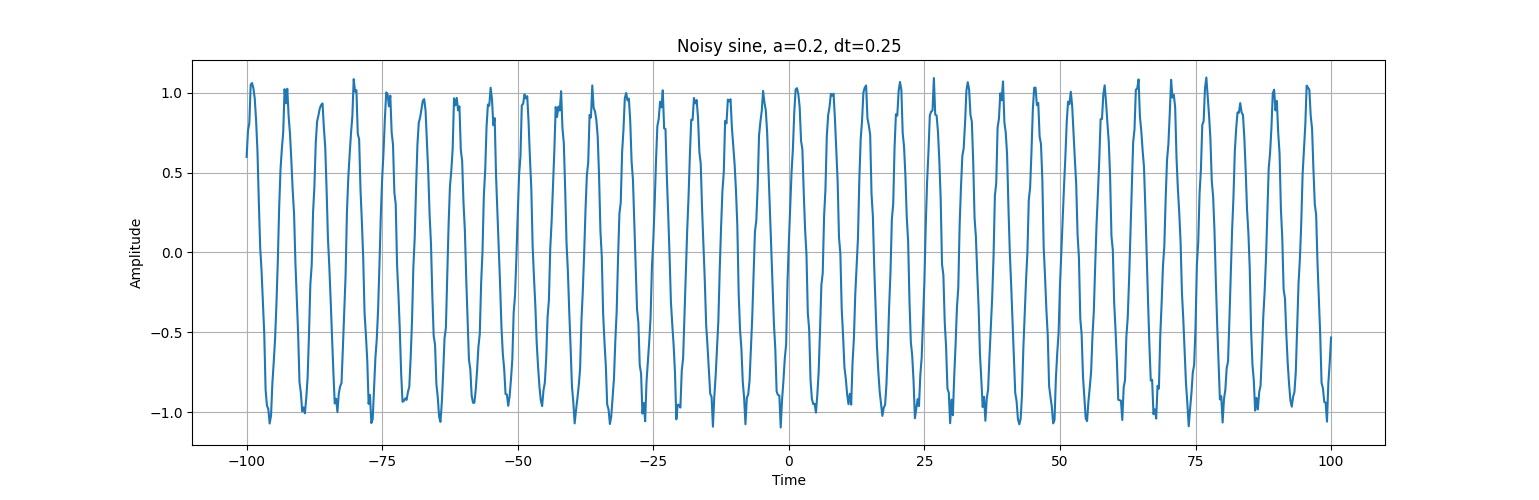
\includegraphics[scale=0.4]{1_noisy_sine.png}
        \captionsetup{skip=0pt}
        \caption{График зашумленного сигнала.}
        \label{fig:1ns}
    \end{figure}
    Найдем численную производную от данного сигнала, используя формулу поэлементного дифференцирования $$\dfrac{y(k+1)-y(k)}{dt},$$ после чего построим график.
    \begin{figure}[H]
        \centering
        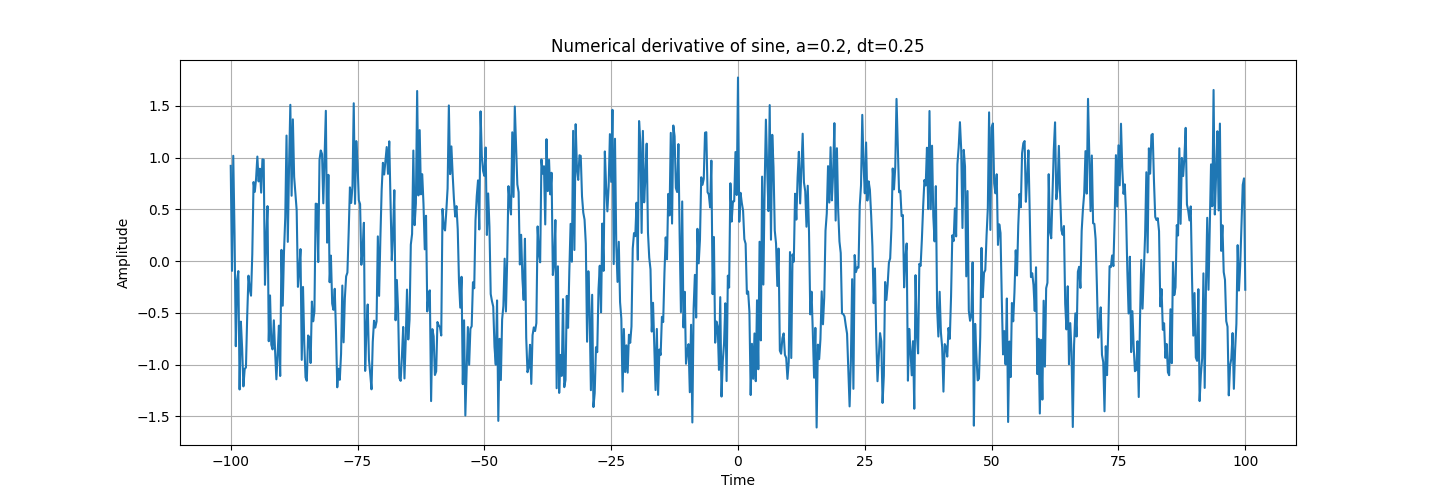
\includegraphics[scale=0.4]{1_numdiff_sine.png}
        \captionsetup{skip=0pt}
        \caption{Численная производная зашумленного сигнала.}
        \label{fig:1nds}
    \end{figure}
    Найдем спектральную производную от зашумленного сигнала. Для прямого и обратного преобразования Фурье будем использовать численное интегрирование (trapz). Чтобы
    превратить Фурье-образ сигнала в Фурье-образ производной, необходимо домножить результат преобразования Фурье на $2\pi i \nu$, где $\nu$ -- частота (Гц),
    таким образом получим формулу $$\mathcal{F}\left\{\frac{d}{dt}f\right\}=2\pi i \nu \mathcal{F}\left\{f\right\}.$$ Теперь остается только выполнить обратное преобразование Фурье, чтобы получить
    спектральную производную сигнала. Далее приведены графики вещественной и мнимой компонент Фурье-образа сигнала и его спектральной производной.
    \begin{figure}[H]
        \centering
        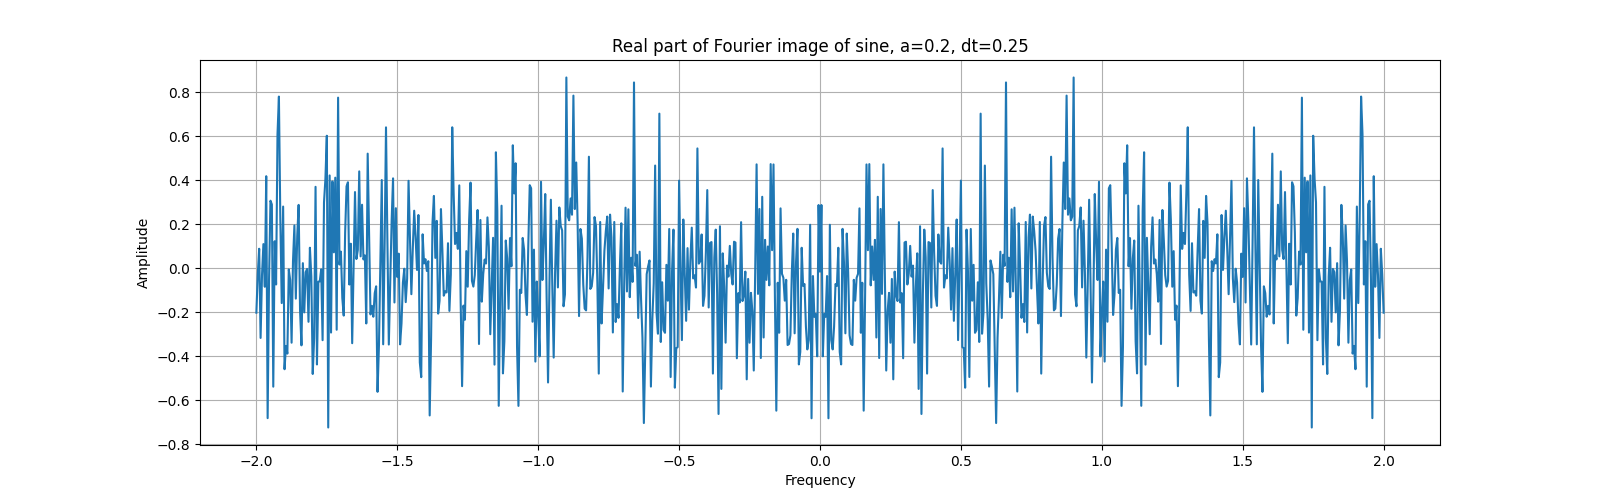
\includegraphics[scale=0.4]{1_re_fimg_sine.png}
        \captionsetup{skip=0pt}
        \caption{Вещественная компонента Фурье-образа зашумленного сигнала.}
        \label{fig:1refis}
    \end{figure}
    \begin{figure}[H]
        \centering
        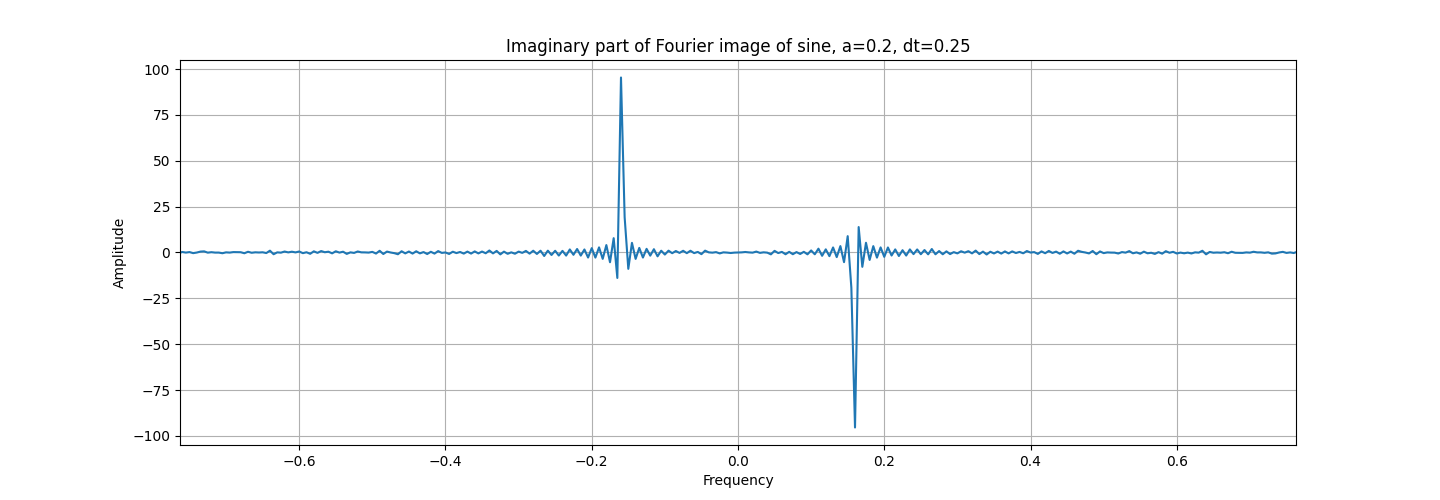
\includegraphics[scale=0.4]{1_im_fimg_sine.png}
        \captionsetup{skip=0pt}
        \caption{Мнимая компонента Фурье-образа зашумленного сигнала.}
        \label{fig:1imfis}
    \end{figure}
    \begin{figure}[H]
        \centering
        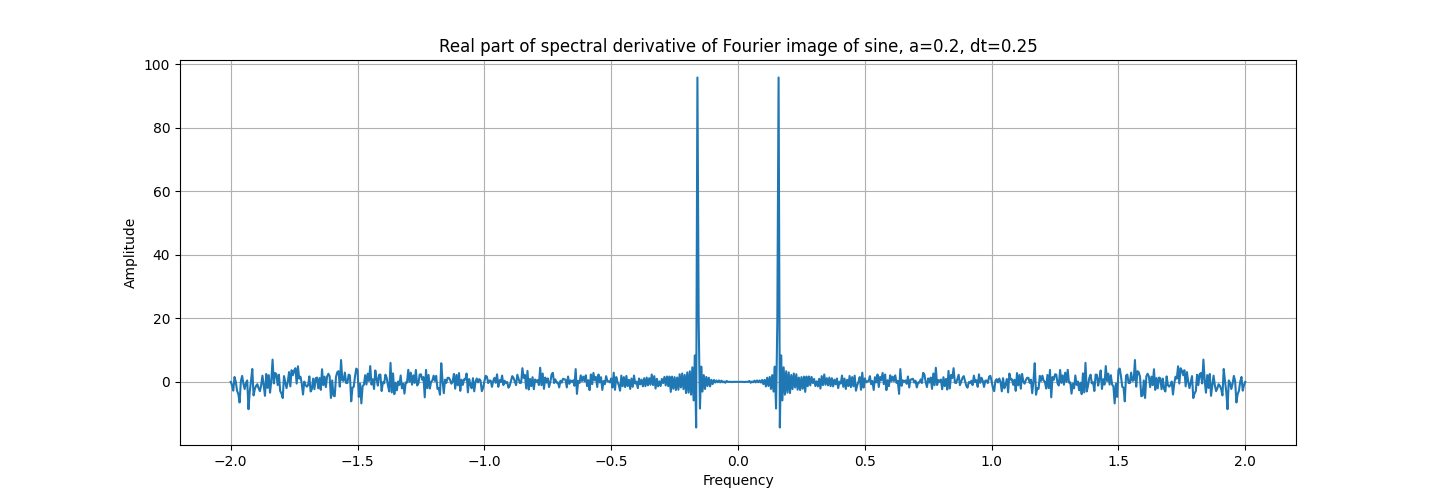
\includegraphics[scale=0.4]{1_re_spd_fimg_sine.png}
        \captionsetup{skip=0pt}
        \caption{Вещественная компонента спектральной производной Фурье-образа зашумленного сигнала.}
        \label{fig:1respdf}
    \end{figure}
    \begin{figure}[H]
        \centering
        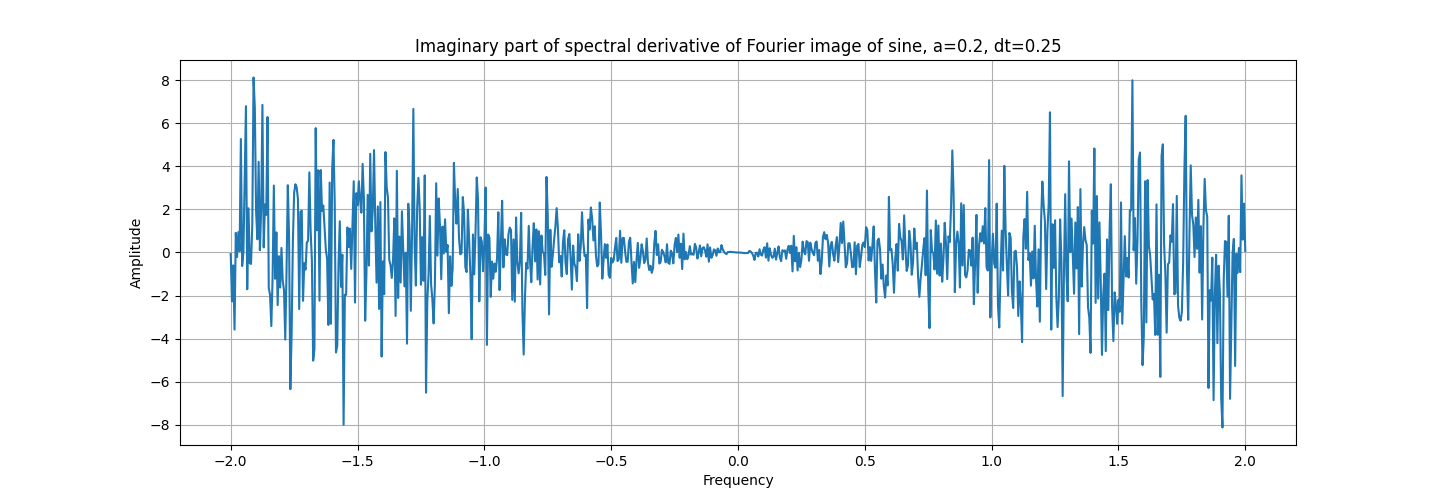
\includegraphics[scale=0.4]{1_im_spd_fimg_sine.png}
        \captionsetup{skip=0pt}
        \caption{Мнимая компонента спектральной производной Фурье-образа зашумленного сигнала.}
        \label{fig:1imspdf}
    \end{figure}


    Видим, что вещественная компонента Фурье-образа зашумленного сигнала и его спектральной производной симметричны относительно оси
    $OY$, а их мнимые компоненты относительно $OX$. Подобная симметричность сохраняется в не зависимости от четности исходной функции.


    На следующем рисунке приведен график вещественной части спектральной производной зашумленного сигнала, найденной с помощью численного интегрирования.
    Результат похож на численную производную, но с резкими возрастаниями амплитуд по краям. Данное поведение не зависит от наличия шума в сигнале или
    выбора шага дискретизации $dt$.
    \begin{figure}[H]
        \centering
        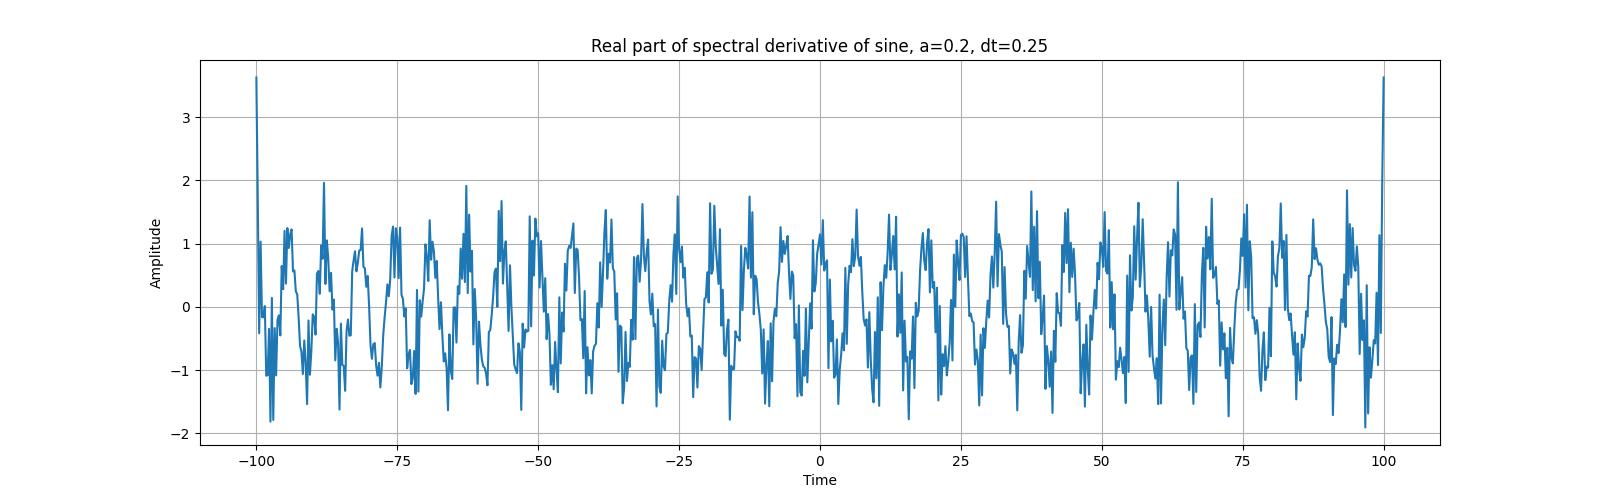
\includegraphics[scale=0.4]{1_re_specdiff_sine.png}
        \captionsetup{skip=0pt}
        \caption{Вещественная компонента спектральной производной зашумленного сигнала.}
        \label{fig:1respds}
    \end{figure}

    
    Теперь сравним график истинной производной $\cos{(t)}$ с графиками численной и спектральной производных зашумленного синуса.
    Оранжевым цветом обозначена спектральная производная, синим численная. Красным цветом выделена производная косинуса.
    \begin{figure}[H]
        \centering
        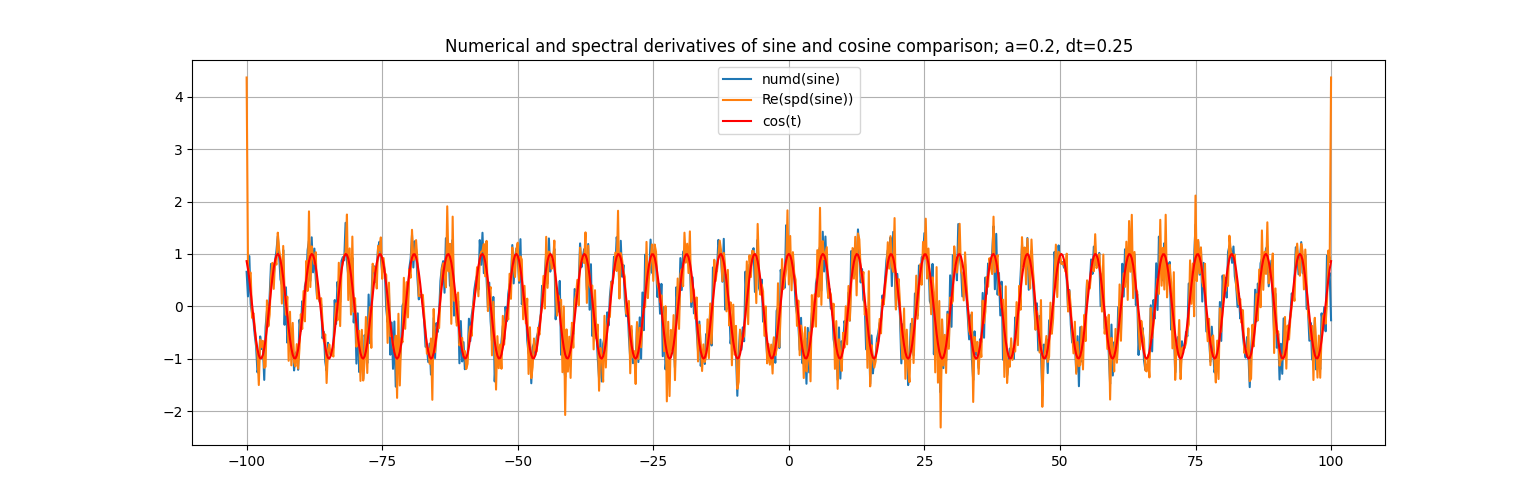
\includegraphics[scale=0.4]{1_css_comp.png}
        \captionsetup{skip=0pt}
        \caption{Сравнительный график производной $\cos{(t)}$ с численной и спектральной производными зашумленного $\sin{(t)}$.}
        \label{fig:css_comp}
    \end{figure}


    Графики численной и спектральной производных похожи друг на друга и на истинную производную косинуса (с разницей в смещении
    по фазе на $-\pi\div 2$). Спектральная производная имеет немного больше выбросов по сравнению с численной. Достаточно посмотреть
    на края графика спектральной производной и на ее амплитуды в точках максимума и минимума каждой волны.


    В ходе работы было выяснено, что при маленьком шаге $dt$ или при большом значении $a$ спектральная и численная производные
    становятся не похожи на истинную производную косинуса. По большей части на графиках видно белый шум. Если исходный сигнал
    имеет шумы, то его производная будет зашумлена сильнее. Наличие мнимой части у Фурье-образа не зависит от четности исходной
    функции. Более того, вещественные компоненты после преобразования Фурье симметричны относительно оси ординат, а мнимые относительно
    оси абсцисс.


    \subsection{Используемые программы}
    Все графики перового задания строились с помощью языка программирования Python с подключенной библиотекой matplotlib. Далее
    по ходу работы графики будут строиться той же программой. 
    \begin{lstlisting}[label=task1, caption={Файл с программой для построения графиков.}]
    import matplotlib.pyplot as plt

    def build_f(x, y, fz1=16,
                fz2=5, clr=None, ttl=None,
                grid=True, legend=False, xlab=None,
                ylab=None, xl1=None, xl2=None,
                yl1=None, yl2=None, lbl=None,
                ls='-', ticks=None, rot=None):
        plt.plot(x, y, color=clr, label=lbl, linestyle=ls)
        plt.xlabel(xlab)
        plt.ylabel(ylab)
        plt.xlim(xl1, xl2)
        plt.ylim(yl1, yl2)
        plt.xticks(ticks, rotation=rot)
        plt.title(ttl)
        plt.gcf().set_size_inches(fz1, fz2)
        plt.grid(grid)
        if legend:
            plt.legend()
        plt.show()
                
    def build_fs(x, y: list, colors: list=None,
                 labels: list=None, fz1=16, fz2=5,
                 ttl=None, grid=True, legend=False, 
                 xlab=None, ylab=None, xl1=None,
                 xl2=None, yl1=None, yl2=None,
                 ls:list=None, ticks=None, rot=None):
        if (y is None or len(y) <= 0):
            print('y is None or its len <= 0')
            return
        if (colors is None): colors = [None] * len(y)
        if (labels is None): labels = [None] * len(y)
        if (ls is None): ls = ['-'] * len(y)
        
        for k in range(len(y)):
            plt.plot(x, y[k], color=colors[k],
                     label=labels[k], linestyle=ls[k])
        plt.xlabel(xlab)
        plt.ylabel(ylab)
        plt.xlim(xl1, xl2)
        plt.ylim(yl1, yl2)
        plt.xticks(ticks, rotation=rot)
        plt.title(ttl)
        plt.gcf().set_size_inches(fz1, fz2)
        plt.grid(grid)
        if legend: plt.legend()
        plt.show()
    \end{lstlisting}


    \newpage
    Для нахождения Фурье-образа и производных использовалась библиотека numpy.
    \begin{lstlisting}[label=task1_2, caption={Программа для вычисления Фурье-образа численным интегрированием и производных.}]
    import numpy as np

    def trapz(y, t, v):
        Y = []
        for k in v:
            Y_k = np.trapz(y * np.exp(-1j * 2 * np.pi * k * t), t)
            Y.append(Y_k)
        return Y

    def undo_trapz(Y, t, v):
        y = []
        for k in t:
            y_k = np.trapz(Y * np.exp(1j * 2 * np.pi * k * v), v)
            y.append(y_k)
        return y

    def numerical_diff(y, dt):
        ndiff = []
        for k in range(len(y) - 1):
            ndiff_k = (y[k + 1] - y[k]) / dt
            ndiff.append(ndiff_k)
        return ndiff

    def spectral_diff(y, t, v):
        Y = trapz(y, t, v)
        dY = 2 * np.pi * 1j * v * Y
        spdiff = undo_trapz(dY, t, v)
        return spdiff, Y, dY
    \end{lstlisting}


    Программа, где используются написанные функции и задаются необходимые параметры, расположена ниже.
    \begin{lstlisting}
    import numpy as np

    import build_func as bf
    import fourier_math as fm

    T = 200
    dt = 0.25
    t = np.arange(-T / 2, T / 2 + dt, dt)
    y = np.sin(t)

    a = 0.2
    y += a * (np.random.rand(len(t)) - 0.5)

    ndsin = fm.numerical_diff(y, dt)
    ndsin.append(y[-1] / 2)

    V = 1 / dt
    dv = 1 / T
    v = np.arange(-V / 2, V / 2 + dv, dv)
    spdsin, Y, dY = fm.spectral_diff(y, t, v)
    tdcos = -np.sin(t)

    bf.build_f(t, y, ttl=f'Noisy sine, a={a}, dt={dt}',
               xlab='Time', ylab='Amplitude')
    bf.build_f(v, np.array(Y).real,
               ttl=f'Real part of Fourier image of sine, a={a}, dt={dt}',
               xlab='Frequency', ylab='Amplitude')
    bf.build_f(v, np.array(Y).imag,
             ttl=f'Imaginary part of Fourier image of sine, a={a}, dt={dt}',
             xlab='Frequency', ylab='Amplitude', xl1=-0.763, xl2=0.763)
    bf.build_f(v, dY.real,
               ttl=f'Real part of spectral derivative of Fourier image of sine, a={a}, dt={dt}',
               xlab='Frequency', ylab='Amplitude')
    bf.build_f(v, dY.imag,
               ttl=f'Imaginary part of spectral derivative of Fourier image of sine, a={a}, dt={dt}',
               xlab='Frequency', ylab='Amplitude')

    bf.build_f(t, ndsin,
               ttl=f'Numerical derivative of sine, a={a}, dt={dt}',
               xlab='Time', ylab='Amplitude')
    bf.build_f(t, np.array(spdsin).real,
            ttl=f'Real part of spectral derivative of sine, a={a}, dt={dt}',
            xlab='Time', ylab='Amplitude')
    bf.build_fs(t, y=[ndsin, np.array(spdsin).real, tdcos],
                colors=[None, None, 'r'], legend=True, 
                labels=['Num. der. of sine', 'Re. spec. der. of sine', 'True der. of cosine'],
                ttl=f'True der. of cosine, num. der. of sine and spec. der. of sine comparison; a={a}, dt={dt}')
    \end{lstlisting}


    \section{Задание 2. Линейные фильтры.}
    Рассмотрим сигнал вида $$u=g+b\cdot(\text{random}(\text{len}(t))-0.5) + c\cdot \sin(d\cdot t),$$ который будем пропускать
    через линейные фильтры.


    \subsection{Фильтр первого порядка.}
    Положим $c=0,\,a=1,\,b=0.6,\,d=0.7$. Будем задавать различные значения постоянной времени $T>0$ и пропускать сигнал через линейный
    фильтр первого порядка $$W_1(p)=\dfrac{1}{Tp+1},$$ после чего построим сравнительные графики и исследуем влияние параметров $T$ и $a$
    на эффективность фильтрации.


    Далее расположены сравнительные графики исходного и фильтрованного сигналов, графики модулей их Фурье-образов, а также АЧХ и ЛАЧХ фильтра.
    В названии графиков указаны значения используемых параметров. Синим цветом обозначаются функции, относящиеся к исходному сигналу, оранжевым
    -- к фильтрованному. Дополнительно на графике во временной области отрисована исходная функция $g(t)$ для более наглядного рассмотрения работы
    фильтрации.
    \begin{figure}[H]
        \centering
        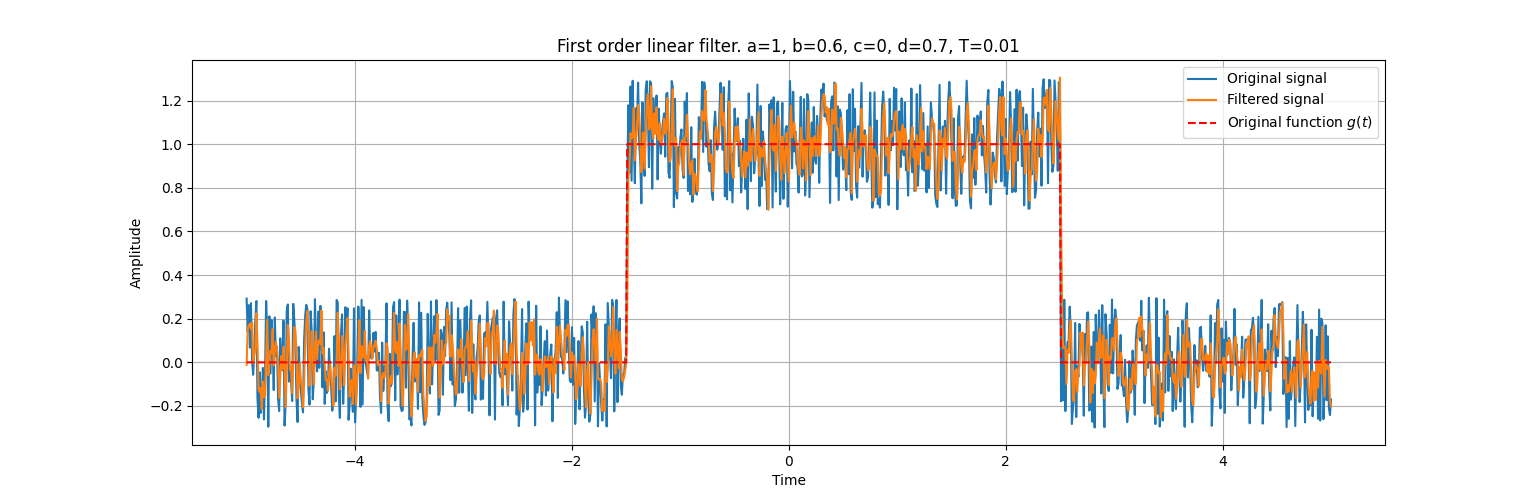
\includegraphics[scale=0.4]{1_filtered_linear.png}
        \captionsetup{skip=0pt}
        \caption{График исходного и фильтрованного сигналов (1).}
        \label{fig:filin1}
    \end{figure}
    \begin{figure}[H]
        \centering
        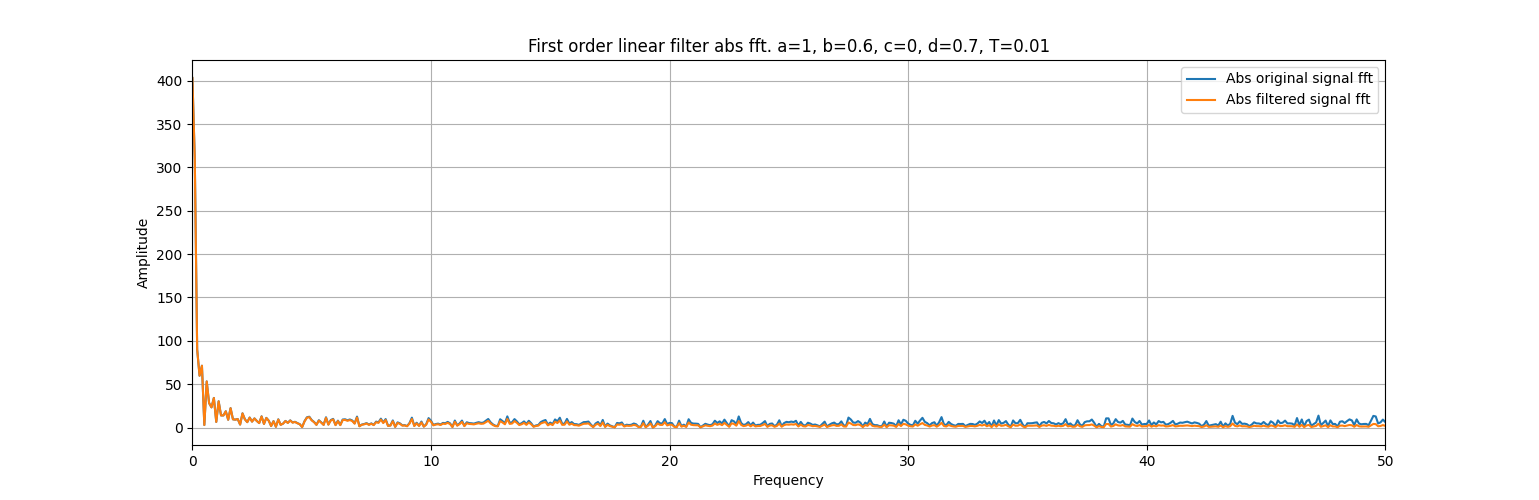
\includegraphics[scale=0.4]{1_abs_filtered_linear.png}
        \captionsetup{skip=0pt}
        \caption{График модулей Фурье-образа исходного и фильтрованного сигналов (1).}
        \label{fig:filinabs1}
    \end{figure}
    \begin{figure}[H]
        \centering
        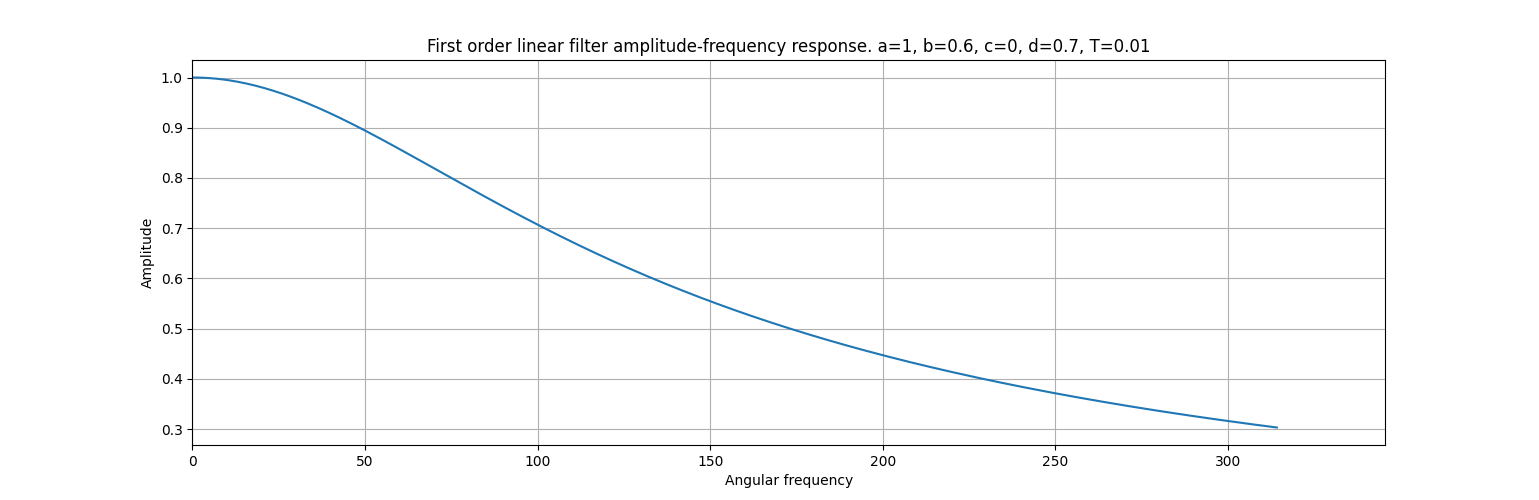
\includegraphics[scale=0.4]{1_afr_filtered_linear.png}
        \captionsetup{skip=0pt}
        \caption{График амплитудно-частотной характеристики фильтра (1).}
        \label{fig:filinafr1}
    \end{figure}
    \begin{figure}[H]
        \centering
        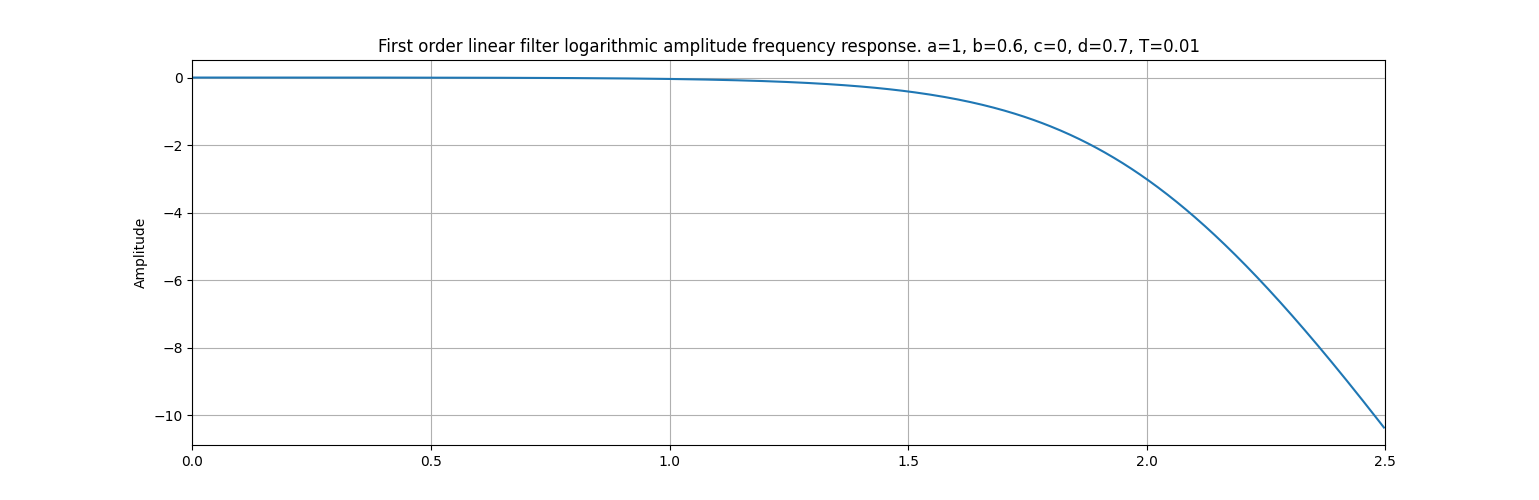
\includegraphics[scale=0.4]{1_lafr_filtered_linear.png}
        \captionsetup{skip=0pt}
        \caption{График логарифмической амплитудно-частотной характеристики фильтра (1).}
        \label{fig:filinlafr1}
    \end{figure}
    \begin{figure}[H]
        \centering
        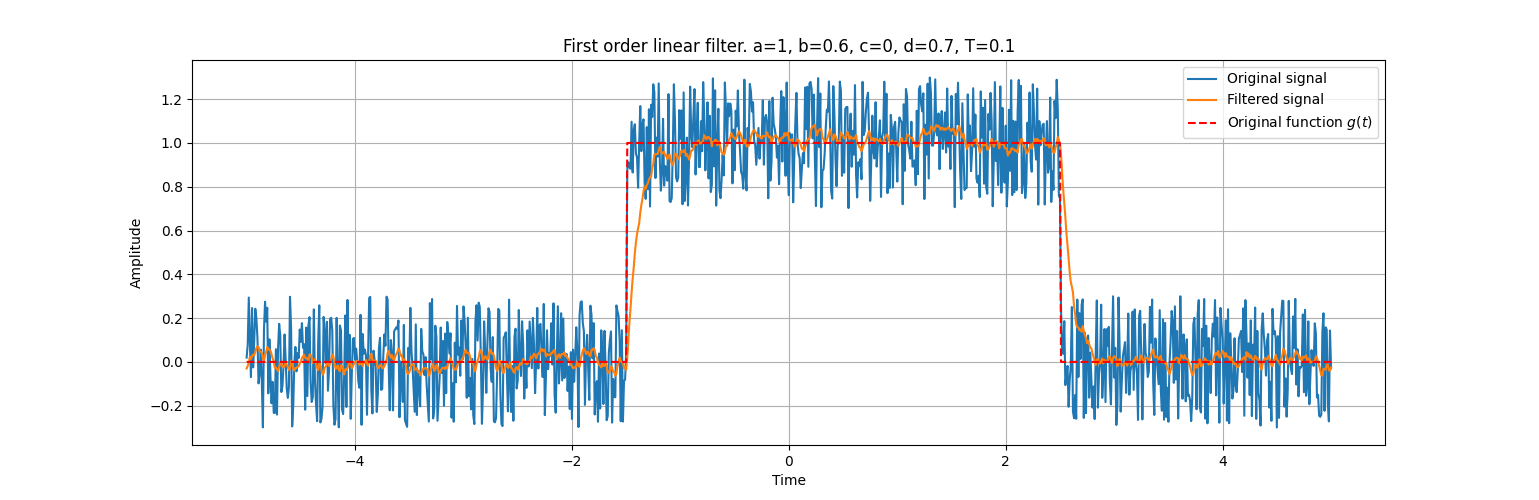
\includegraphics[scale=0.4]{2_filtered_linear.png}
        \captionsetup{skip=0pt}
        \caption{График исходного и фильтрованного сигналов (2).}
        \label{fig:filin11}
    \end{figure}
    \begin{figure}[H]
        \centering
        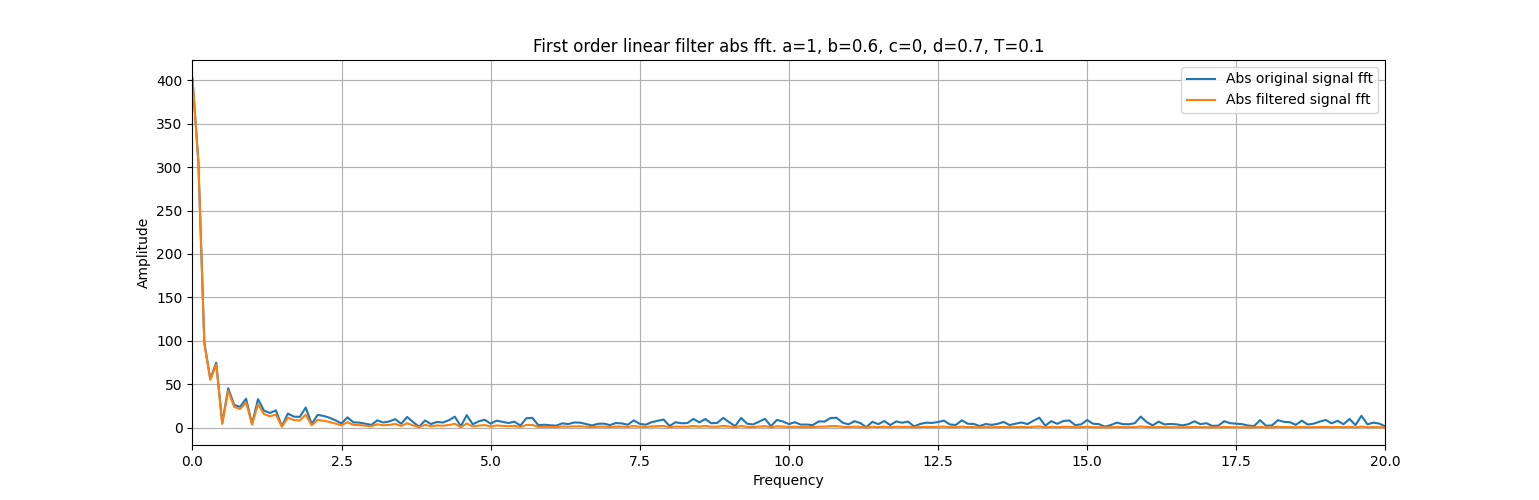
\includegraphics[scale=0.4]{2_abs_filtered_linear.png}
        \captionsetup{skip=0pt}
        \caption{График модулей Фурье-образа исходного и фильтрованного сигналов (2).}
        \label{fig:filinabs11}
    \end{figure}
    \begin{figure}[H]
        \centering
        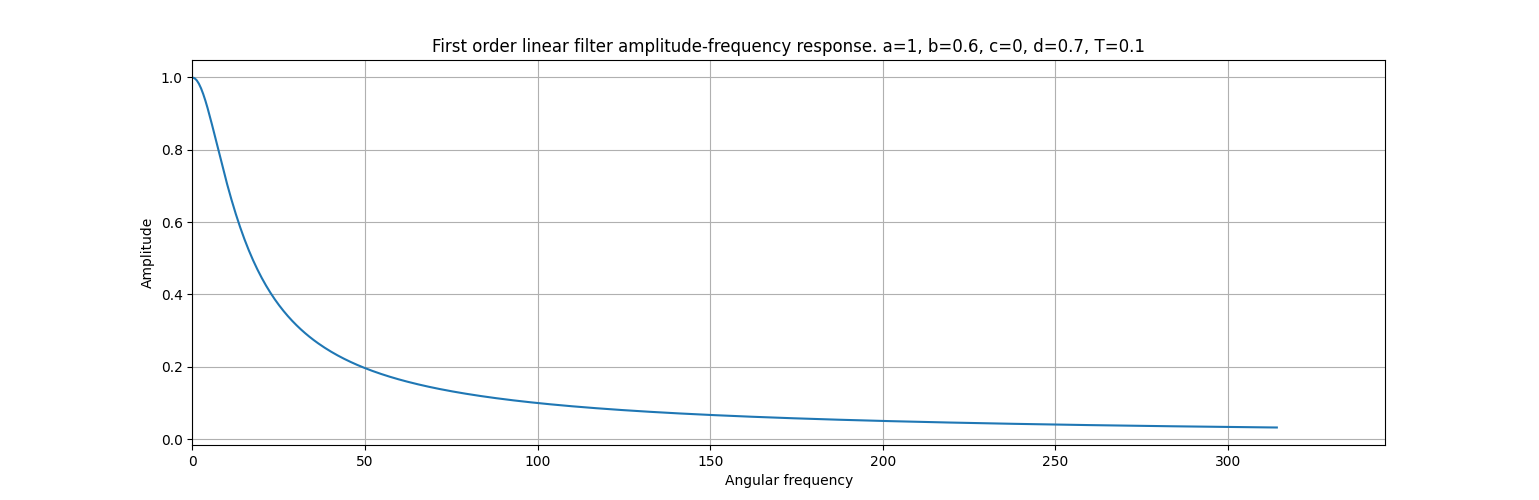
\includegraphics[scale=0.4]{2_afr_filtered_linear.png}
        \captionsetup{skip=0pt}
        \caption{График амплитудно-частотной характеристики фильтра (2).}
        \label{fig:filinafr11}
    \end{figure}
    \begin{figure}[H]
        \centering
        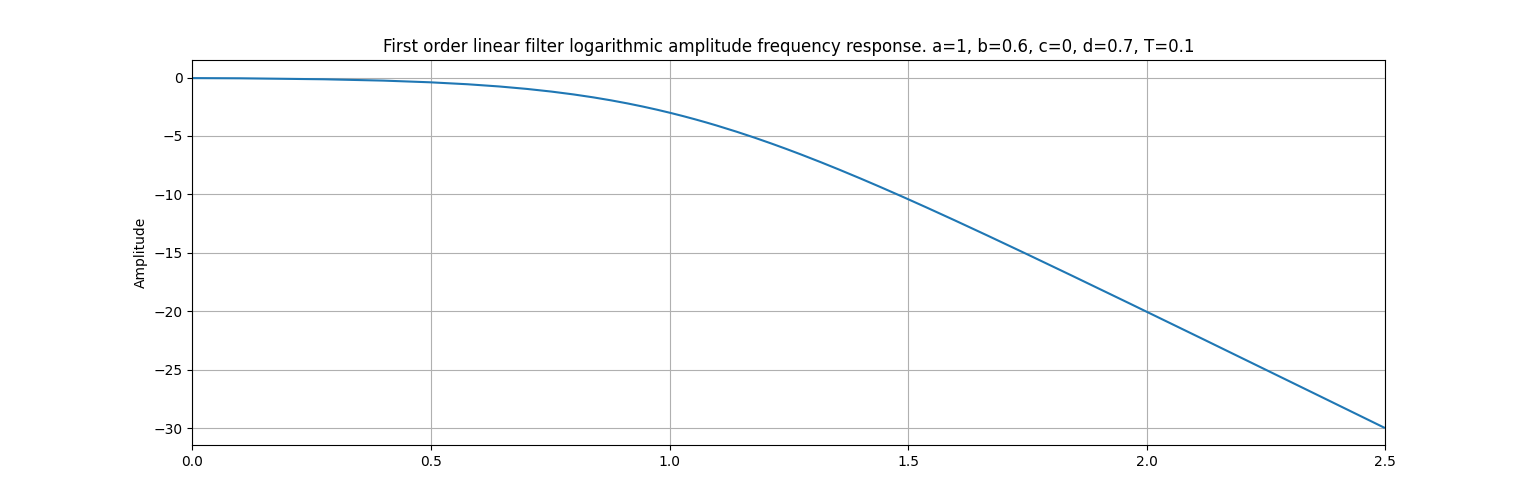
\includegraphics[scale=0.4]{2_lafr_filtered_linear.png}
        \captionsetup{skip=0pt}
        \caption{График логарифмической амплитудно-частотной характеристики фильтра (2).}
        \label{fig:filinlafr11}
    \end{figure}
    \begin{figure}[H]
        \centering
        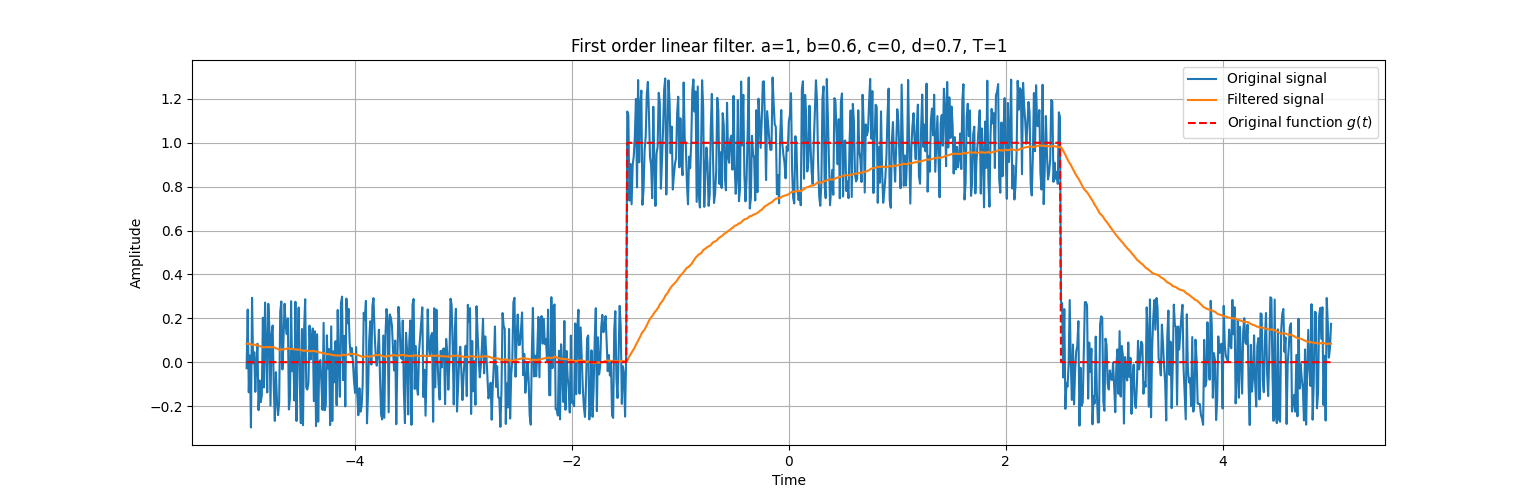
\includegraphics[scale=0.4]{3_filtered_linear.png}
        \captionsetup{skip=0pt}
        \caption{График исходного и фильтрованного сигналов (3).}
        \label{fig:filin13}
    \end{figure}
    \begin{figure}[H]
        \centering
        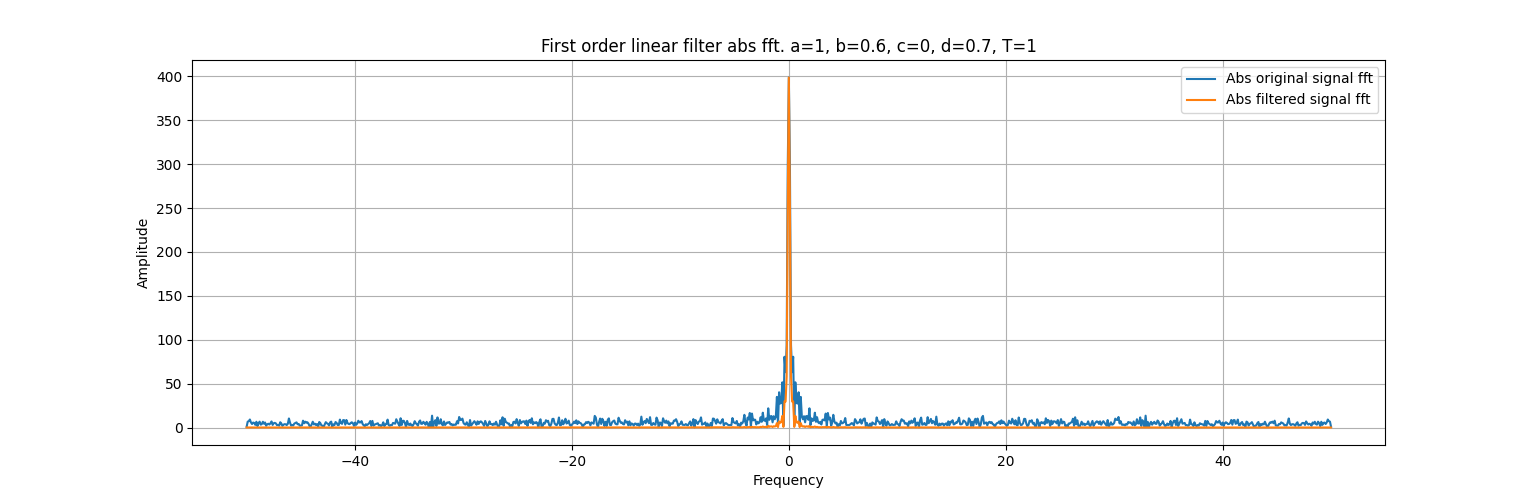
\includegraphics[scale=0.4]{3_abs_filtered_linear.png}
        \captionsetup{skip=0pt}
        \caption{График модулей Фурье-образа исходного и фильтрованного сигналов (3).}
        \label{fig:filinabs13}
    \end{figure}
    \begin{figure}[H]
        \centering
        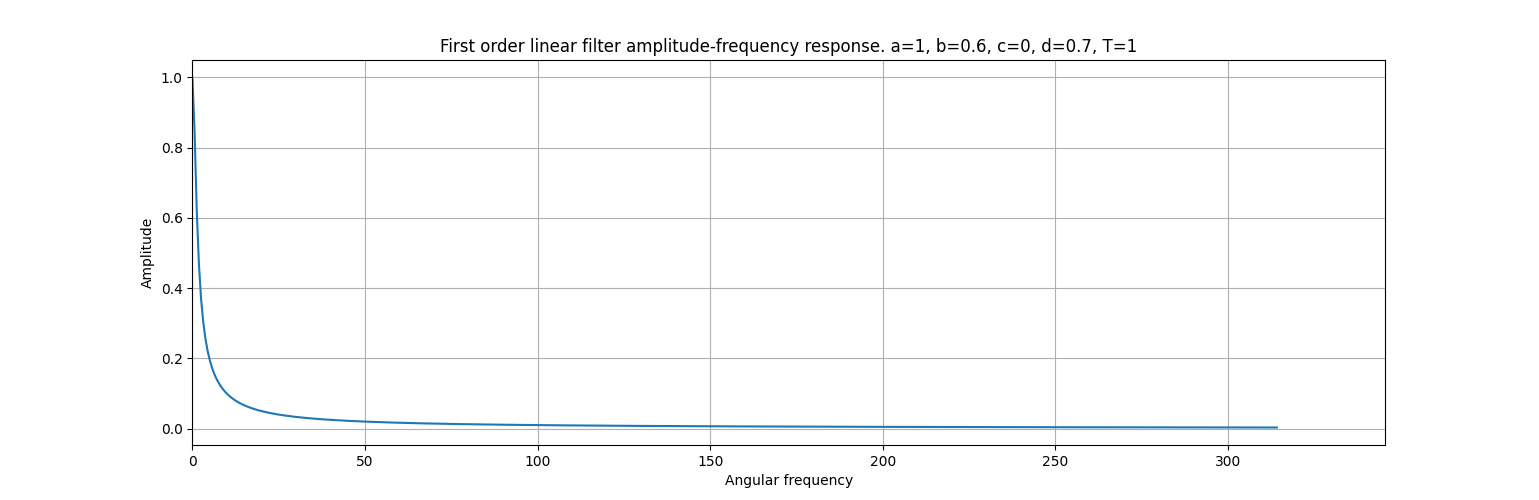
\includegraphics[scale=0.4]{3_afr_filtered_linear.png}
        \captionsetup{skip=0pt}
        \caption{График амплитудно-частотной характеристики фильтра (3).}
        \label{fig:filinafr13}
    \end{figure}
    \begin{figure}[H]
        \centering
        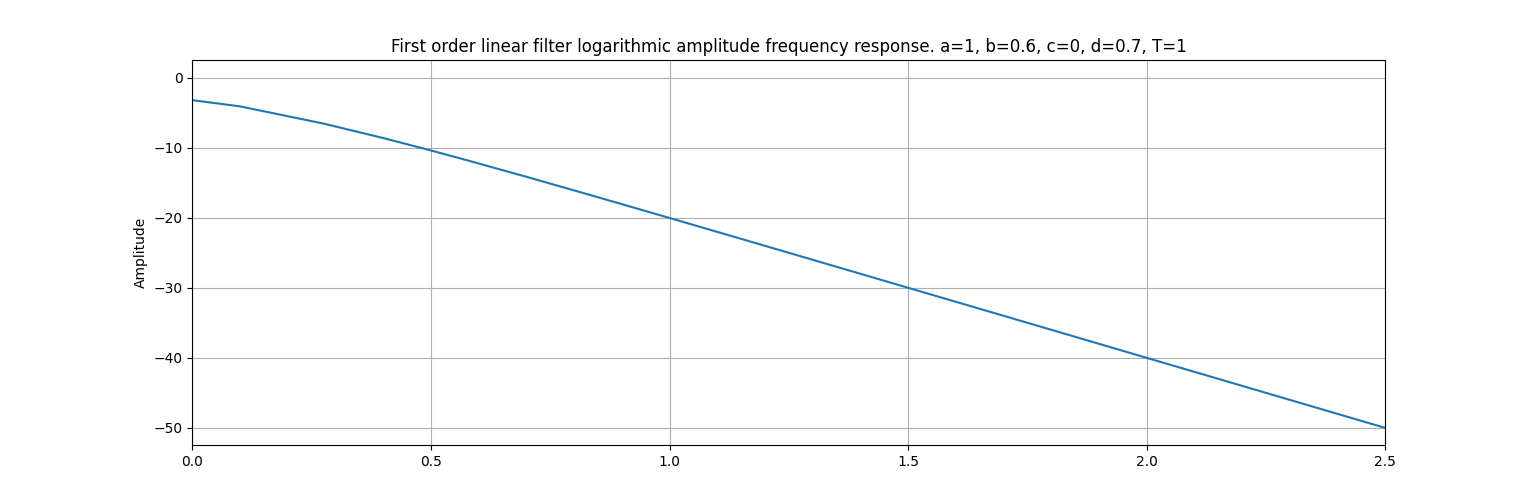
\includegraphics[scale=0.4]{3_lafr_filtered_linear.png}
        \captionsetup{skip=0pt}
        \caption{График логарифмической амплитудно-частотной характеристики фильтра (3).}
        \label{fig:filinlafr13}
    \end{figure}
    \begin{figure}[H]
        \centering
        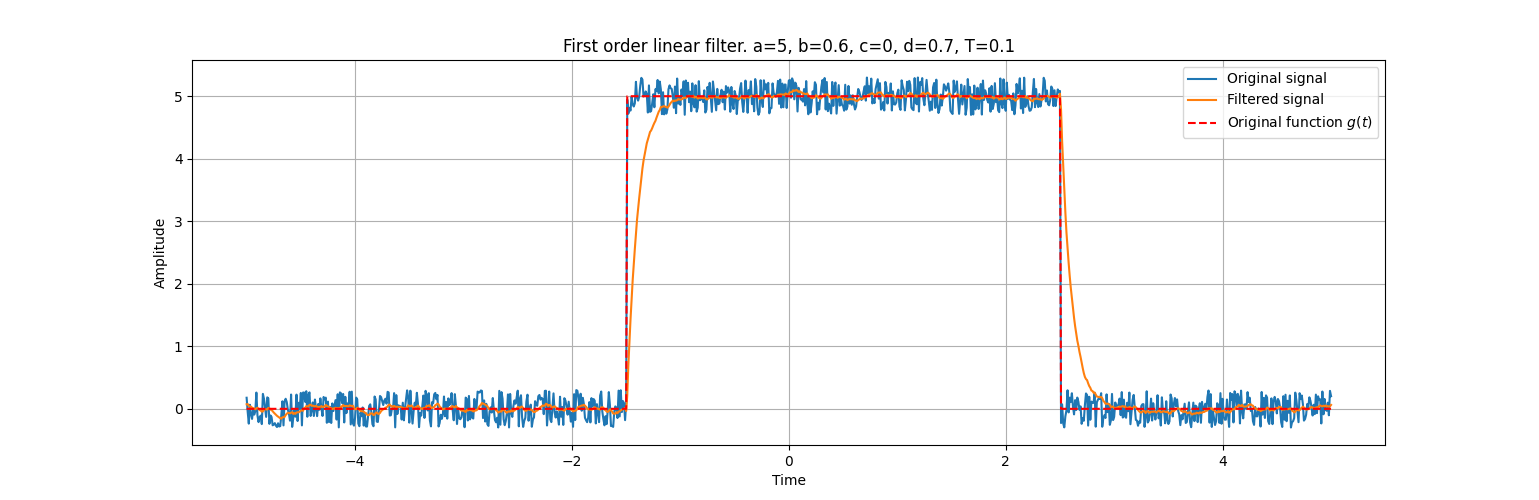
\includegraphics[scale=0.4]{4_filtered_linear.png}
        \captionsetup{skip=0pt}
        \caption{График исходного и фильтрованного сигналов (4).}
        \label{fig:filin14}
    \end{figure}
    \begin{figure}[H]
        \centering
        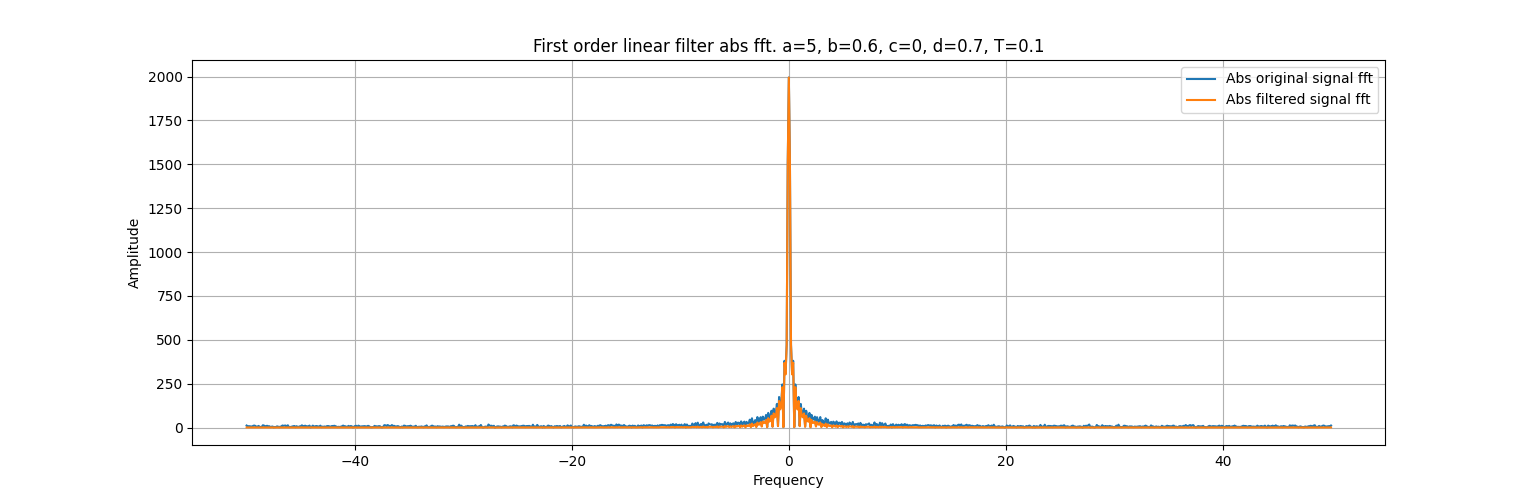
\includegraphics[scale=0.4]{4_abs_filtered_linear.png}
        \captionsetup{skip=0pt}
        \caption{График модулей Фурье-образа исходного и фильтрованного сигналов (4).}
        \label{fig:filinabs14}
    \end{figure}
    \begin{figure}[H]
        \centering
        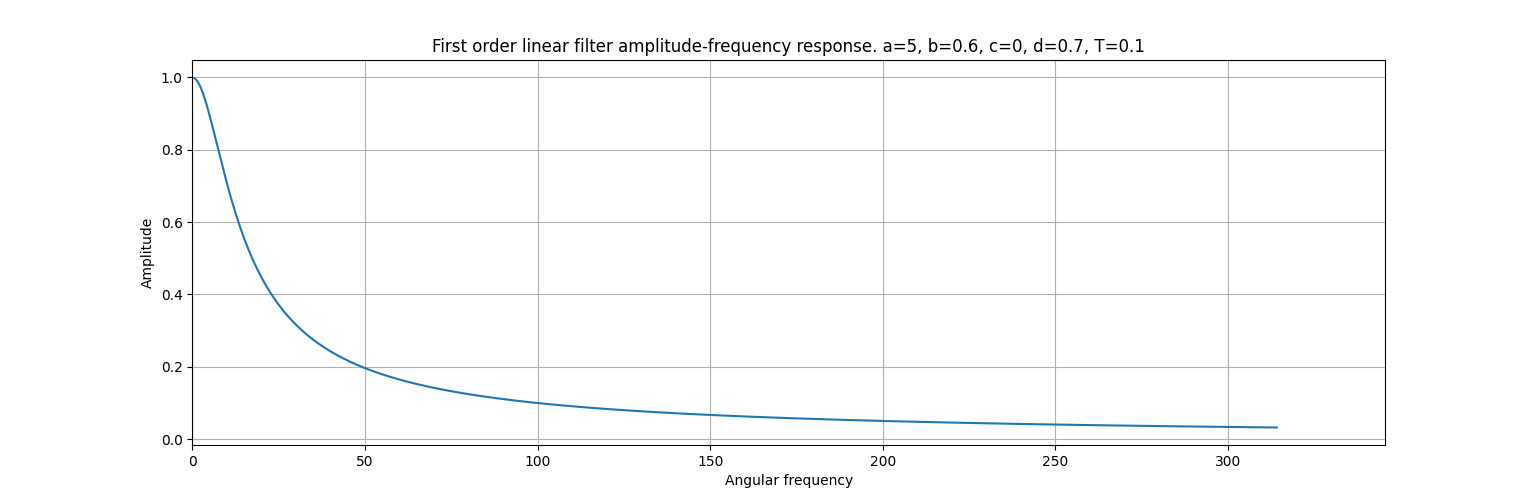
\includegraphics[scale=0.4]{4_afr_filtered_linear.png}
        \captionsetup{skip=0pt}
        \caption{График амплитудно-частотной характеристики фильтра (4).}
        \label{fig:filinafr14}
    \end{figure}
    \begin{figure}[H]
        \centering
        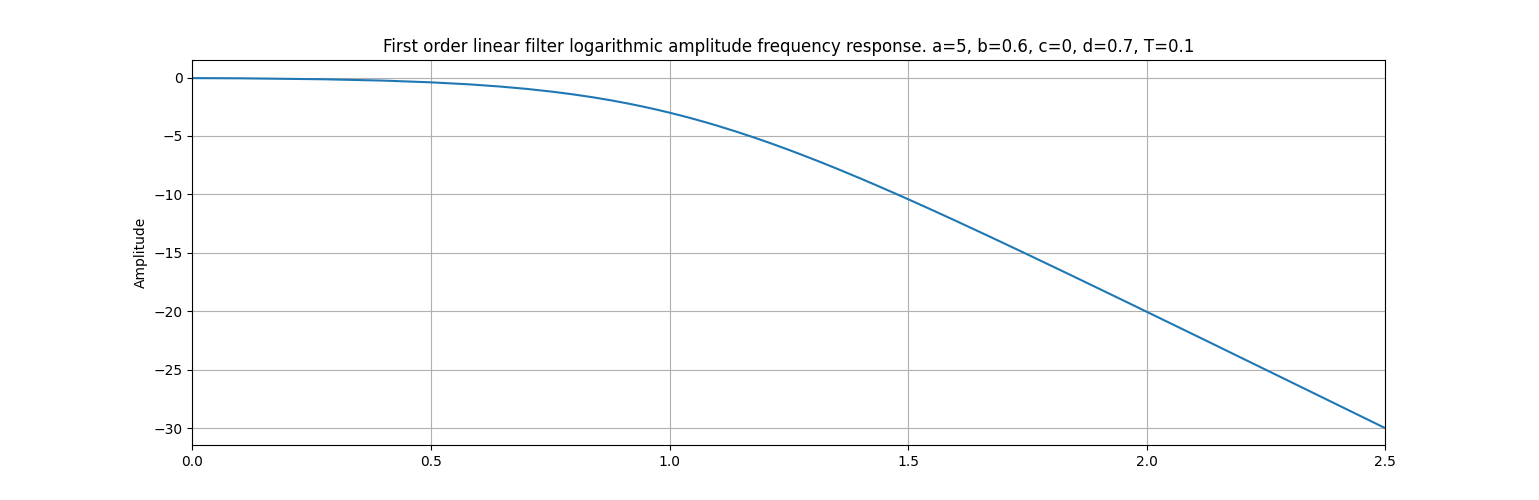
\includegraphics[scale=0.4]{4_lafr_filtered_linear.png}
        \captionsetup{skip=0pt}
        \caption{График логарифмической амплитудно-частотной характеристики фильтра (4).}
        \label{fig:filinlafr14}
    \end{figure}
    \begin{figure}[H]
        \centering
        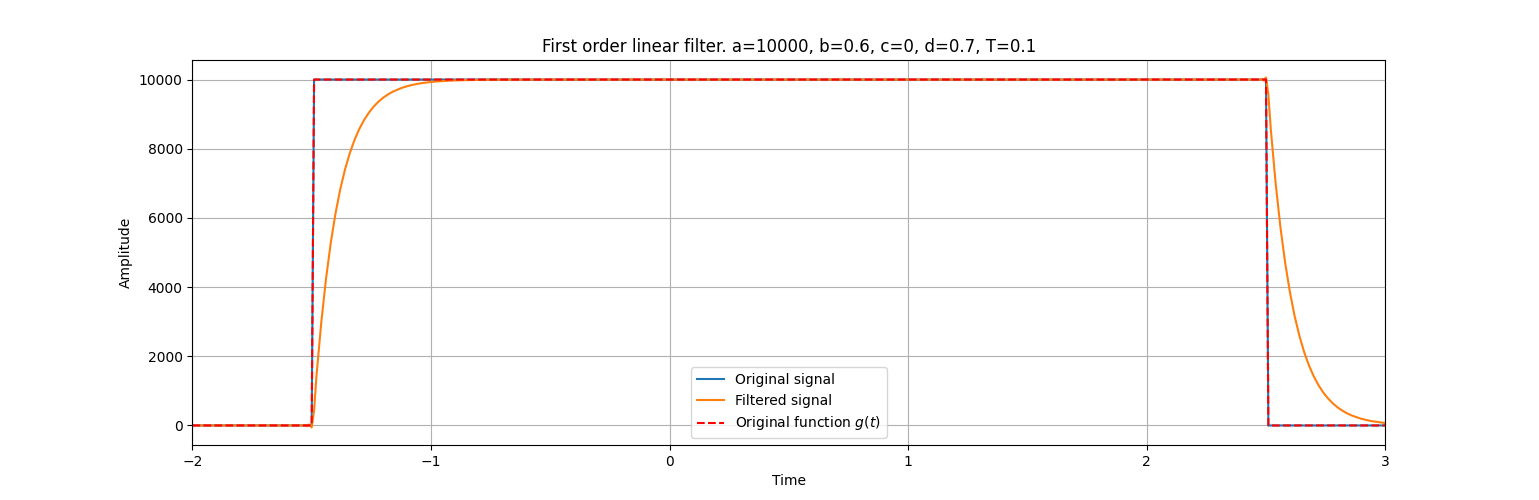
\includegraphics[scale=0.4]{alin1.png}
        \captionsetup{skip=0pt}
        \caption{Более детальное исследование параметра $a$ (Исходный и фильтрованный сигнал).}
        \label{fig:alin1}
    \end{figure}
    \begin{figure}[H]
        \centering
        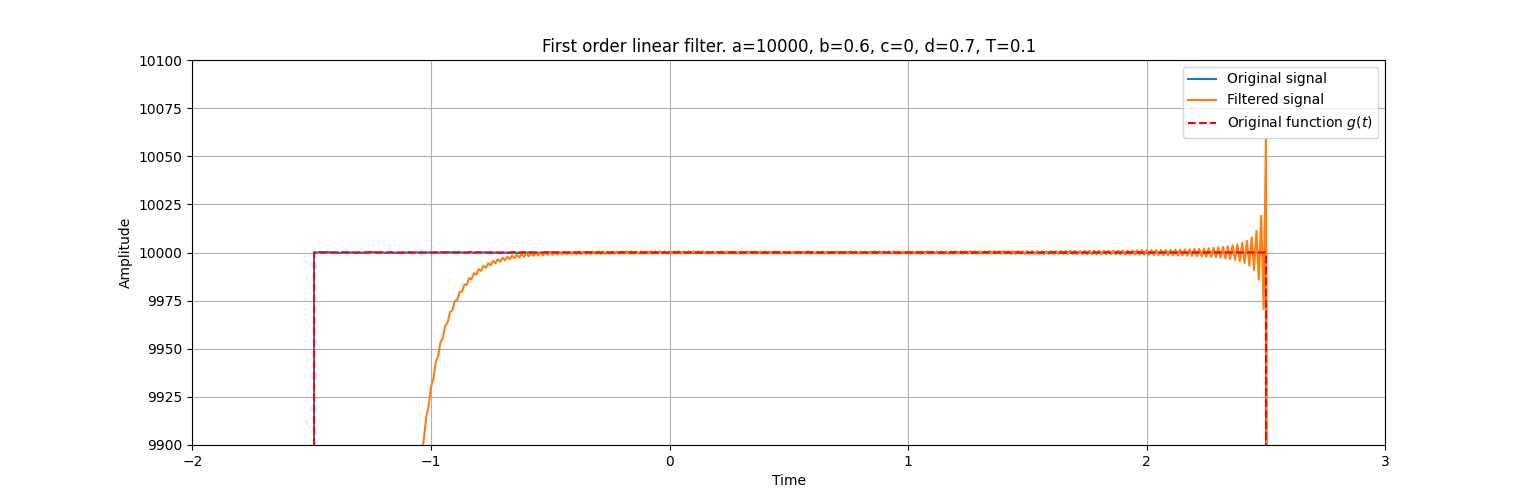
\includegraphics[scale=0.4]{alin2.png}
        \captionsetup{skip=0pt}
        \caption{Более детальное исследование параметра $a$ (Поднятая часть сигналов в приближении).}
        \label{fig:alin2}
    \end{figure}
    \begin{figure}[H]
        \centering
        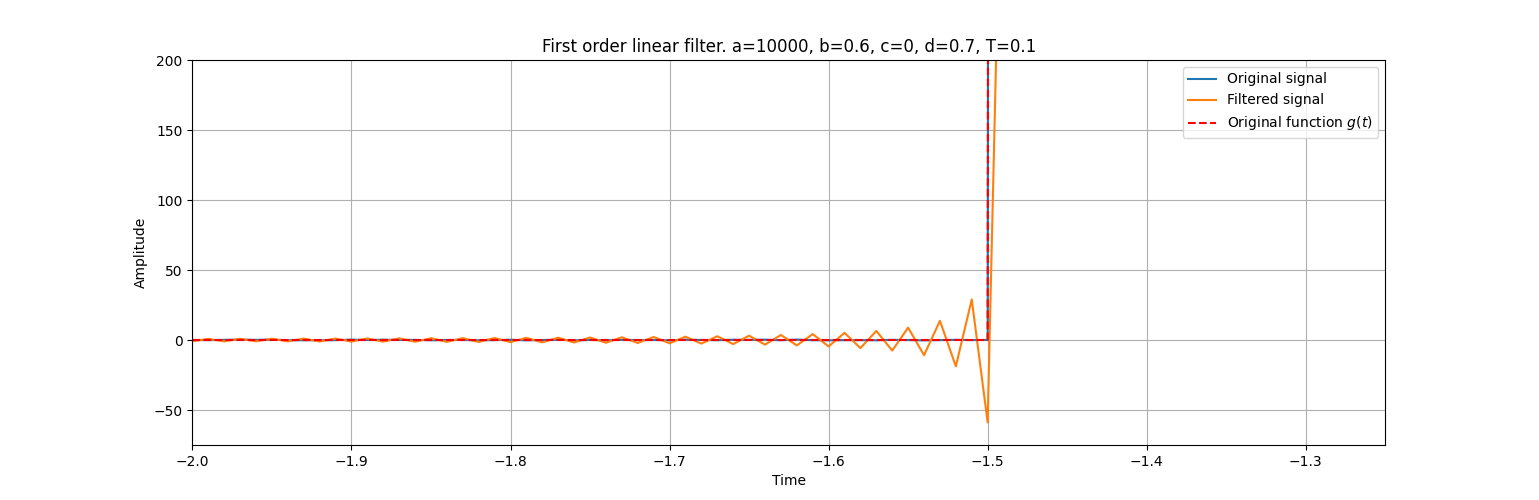
\includegraphics[scale=0.4]{alin3.png}
        \captionsetup{skip=0pt}
        \caption{Более детальное исследование параметра $a$ (Левый разрыв сигналов).}
        \label{fig:alin3}
    \end{figure}
    \begin{figure}[H]
        \centering
        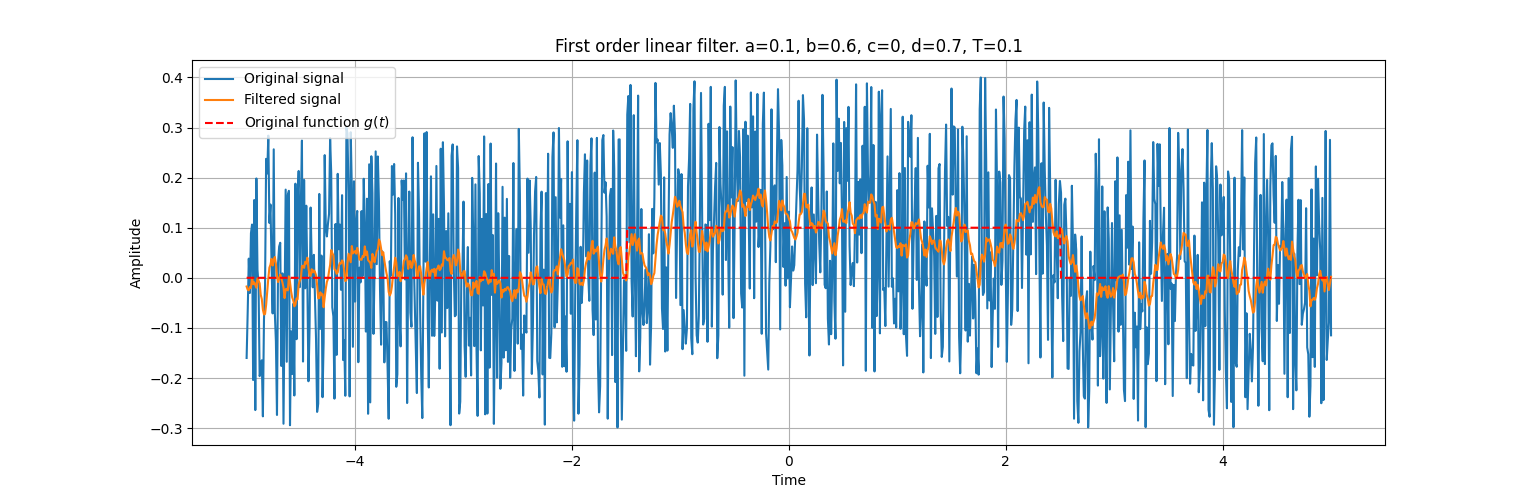
\includegraphics[scale=0.4]{alin4.png}
        \captionsetup{skip=0pt}
        \caption{Более детальное исследование параметра $a$.}
        \label{fig:alin4}
    \end{figure}


    Исходя из графиков можно сделать вывод, что при маленьких и больших значениях постоянной времени $T$ фильтрация хуже,
    чем при средних значениях. Большие значения приводят к излишей фильтрации сигнала -- результирующий сигнал хоть и хорошо
    сглажен, но приобрел лишний наклон (см. рис. \ref{fig:filin13}). На рис. \ref{fig:filinabs13} видно, что в некотором
    небольшом диапазоне нуля большинство важных частот (имеющих б\'{о}льшие амплитуды по сравнению с другими) урезалось
    фильтром. Еще лучше это видно на графике АЧХ -- частота среза по оси абсцисс находится близко к оси ординат, что означает,
    что фильтр оставил немного амплитуд, соответствующих нижним частотам, нетронутыми, а ниже частоты среза график быстро убывает
    -- происходит резкое ослабление амплитуд соответствующих частот (см. рис. \ref{fig:filinafr13}). Маленькие значения приводят к
    недостаточной фильтрации сигнала -- хотя фильтрованный сигнал и выглядит лучше исходного, осталось много белого шума
    (см. рис. \ref{fig:filin1}). На графике модулей Фурье-образов большинство менее значимых частот было оставлено
    (см. рис. \ref{fig:filinabs1}). На графике АЧХ рисунка \ref{fig:filinafr1} хорошо видно, что частота среза
    находится примерно в точке $\left(\omega_0=100,\,A=1\div\sqrt{2}\right)$, и, ослабление амплитуд ниже такой частоты среза несильное
    (график медленно убывает). На графике ЛАЧХ частота среза находится примерно в точке $\left(2,\,-3\right)$ (см. рис. \ref{fig:filinlafr1}).
    На графиках ЛАЧХ (см. рис. \ref{fig:filinlafr1}, \ref{fig:filinlafr11}, \ref{fig:filinlafr13})
    при последовательном увеличении значения $T$ с каждым разом частота среза приближается к нижним частотам, уменьшаясь в 10 раз при
    переводе из логарифмической шкалы частот (изменение на 1 на логарифмической шкале частот соответствует изменению частоты в 10 раз).
    Примерно это мы и видим на графиках АЧХ -- рис. \ref{fig:filinafr1} $\omega_0\approx 100$, рис. \ref{fig:filinafr11} $\omega_0\approx 10$,
    рис. \ref{fig:filinafr13} $\omega_0\approx 1$. Хорошо фильтрация получилась на рис. \ref{fig:filin11} -- большая часть белого шума пропала,
    график не сильно отклонился и неплохо повторяет функцию $g(t)$.
    
    
    Рассматривая рисунки \ref{fig:filin11}, \ref{fig:filin14} и \ref{fig:alin1} кажется, что
    влияние параметра $a$ на эффективность фильтрации заключается в ее сглаживании -- чем больше значение $a$, тем более гладким становится фильтрованный сигнал.
    Однако по рис. \ref{fig:alin2} и \ref{fig:alin3} можно увидеть, что при большом значении $a$ усиливается эффект Гиббса в местах разрыва сигнала, при этом
    чем ближе сигнал к месту разрыва, тем постепенно больше становятся амплитуды фильтрованного сигнала -- фильтрация явно ухудшается. Также при слишком маленьком
    значении параметра $a$ фильтрованный сигнал выглядит хуже при том же значении параметра $T$ (см. рис. \ref{fig:alin4}, \ref{fig:filin11}). Следовательно, параметр
    $a$ так же как и параметр $T$ следует выбирать не маленьким и не большим.


    \subsection{Специальный фильтр.}
    Положим $b=0$. Рассмотрим линейный фильтр вида
    $$W_2(p)=\dfrac{\left(T_1p+1\right)^{2}}{\left(T_2p+1\right)\left(T_3p+1\right)}=\dfrac{T_1^2p^2+2T_1p+1}{T_2T_3p^2+\left(T_2+T_3\right)p+1},$$
    при этом постараемся подобрать такие $T_1,T_2,T_3>0$, чтобы они по возможности хорошо убирали синусоидальную составляющую помехи и не сильно искажали
    полезный сигнал. Также рассмотрим несколько значений параметра $d$ и найдем подходящие $T_1,T_2,T_3$ для каждого случая. После построим сравнительные
    графики и проанализируем влияние параметра $c$ на эффективность фильтрации.


    Далее расположены сравнительные графики исходного и фильтрованного сигналов, графики модулей их Фурье-образов и АЧХ и ЛАЧХ фильтра.
    Синим цветом отрисованы функции, связанные с исходным сигналом, оранжевым -- с фильтрованным. Также на графике во временной области
    отображена исходная функция $g(t)$.
    \begin{figure}[H]
        \centering
        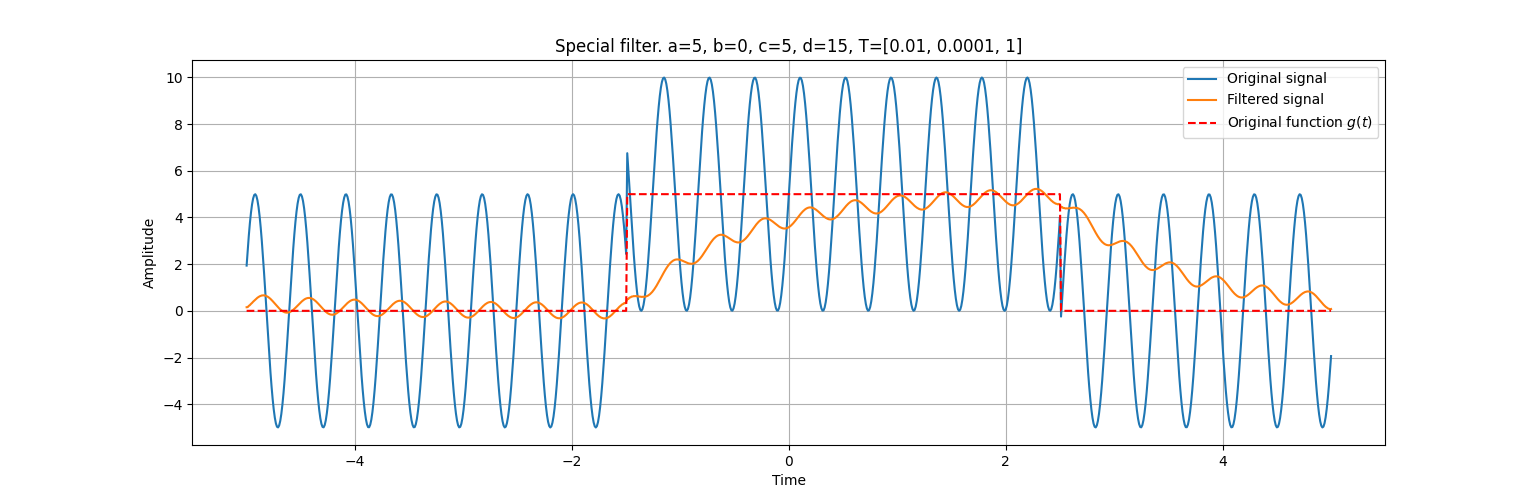
\includegraphics[scale=0.4]{1_fl2.png}
        \captionsetup{skip=0pt}
        \caption{График исходного и фильтрованного сигналов (1).}
        \label{fig:filin21}
    \end{figure}
    \begin{figure}[H]
        \centering
        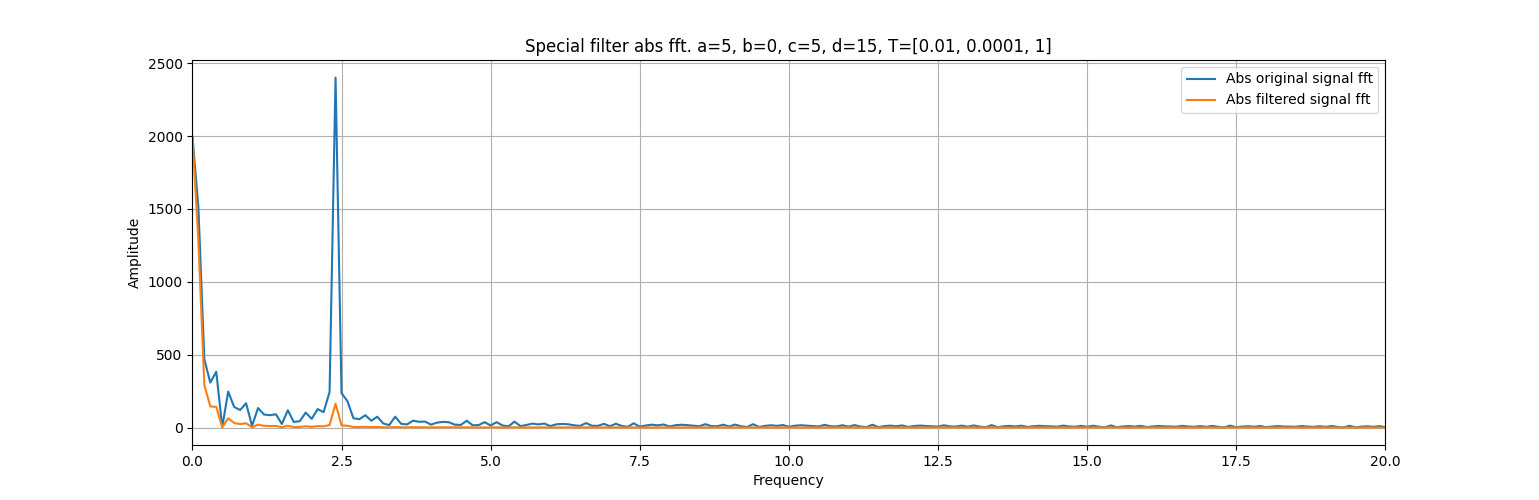
\includegraphics[scale=0.4]{1_fl2_abs.png}
        \captionsetup{skip=0pt}
        \caption{График модулей Фурье-образа исходного и фильтрованного сигналов (1).}
        \label{fig:filinabs21}
    \end{figure}
    \begin{figure}[H]
        \centering
        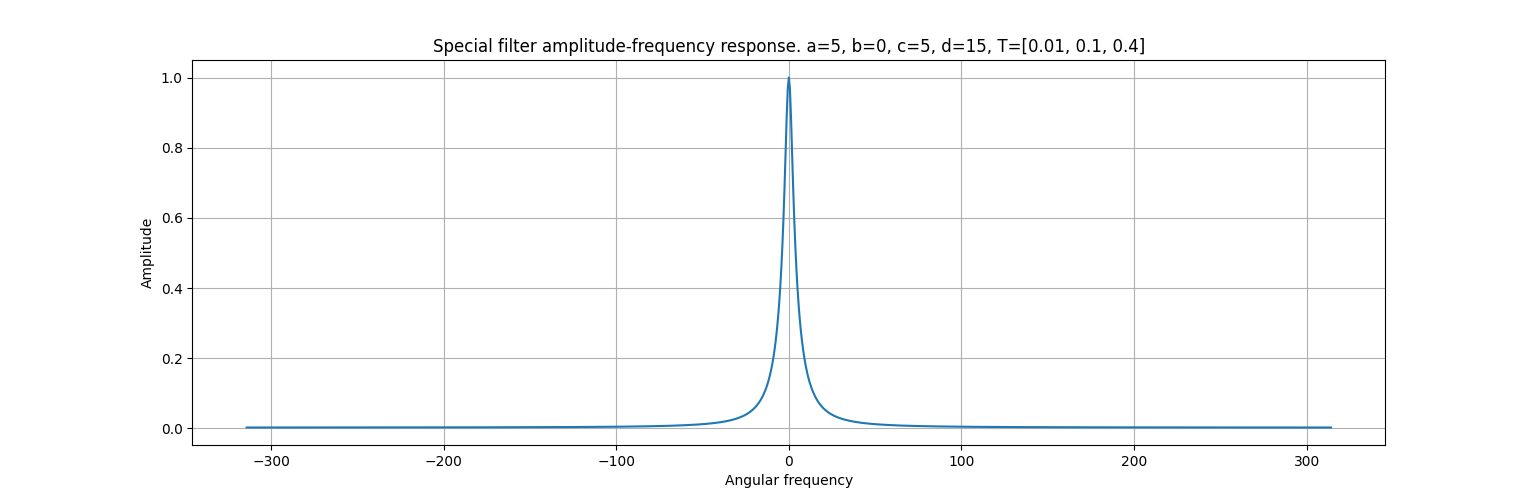
\includegraphics[scale=0.4]{1_fl2_afr.png}
        \captionsetup{skip=0pt}
        \caption{График амплитудно-частотной характеристики фильтра (1).}
        \label{fig:filinafr21}
    \end{figure}
    \begin{figure}[H]
        \centering
        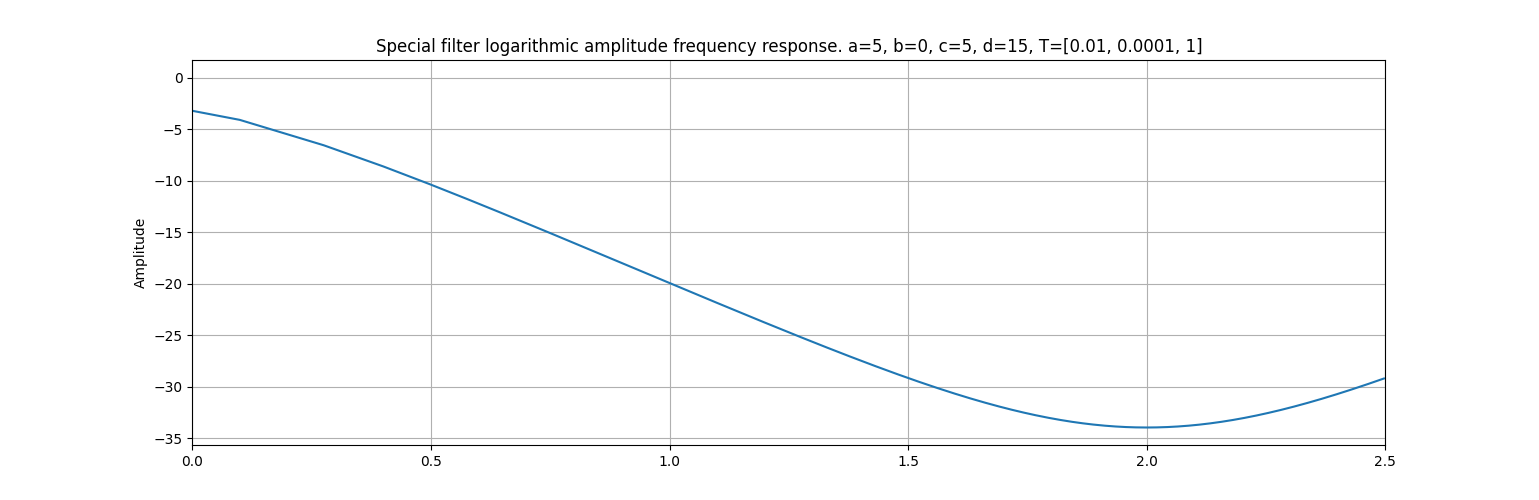
\includegraphics[scale=0.4]{1_fl2_lafr.png}
        \captionsetup{skip=0pt}
        \caption{График логарифмической амплитудно-частотной характеристики фильтра (1).}
        \label{fig:filinlafr21}
    \end{figure}
    \begin{figure}[H]
        \centering
        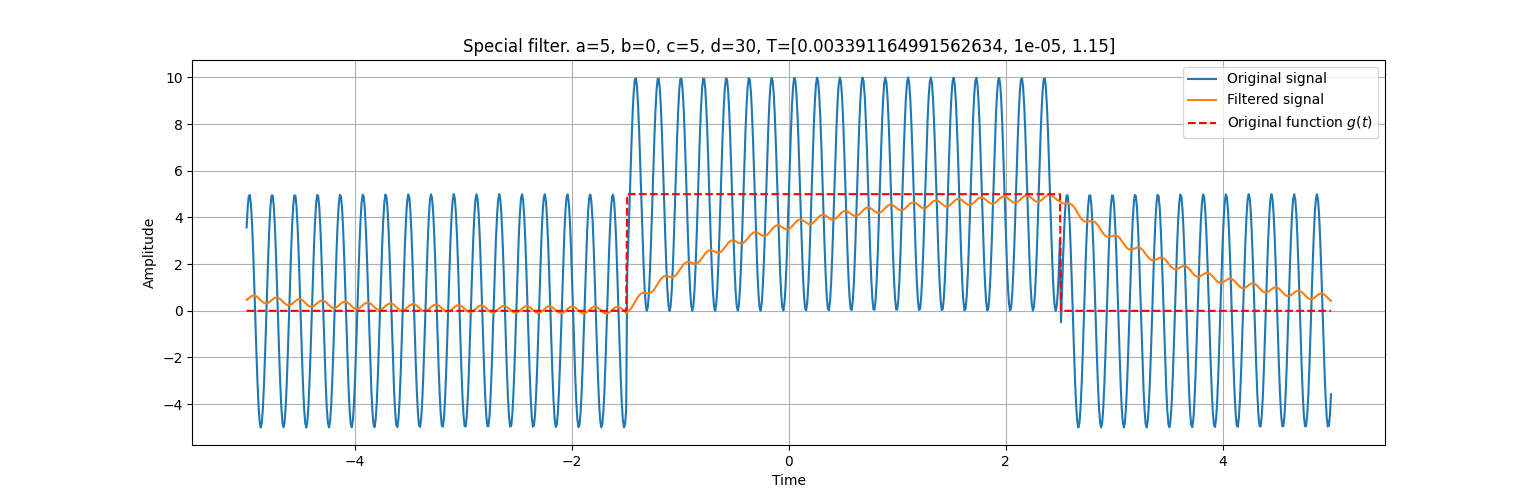
\includegraphics[scale=0.4]{2_fl2.png}
        \captionsetup{skip=0pt}
        \caption{График исходного и фильтрованного сигналов (2).}
        \label{fig:filin22}
    \end{figure}
    \begin{figure}[H]
        \centering
        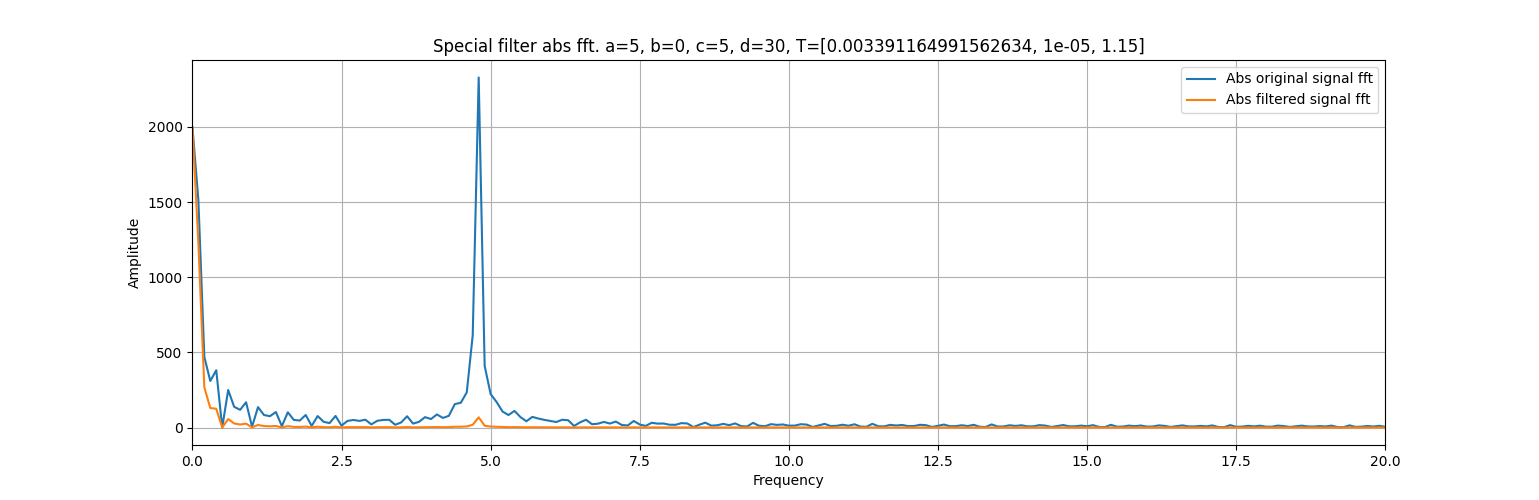
\includegraphics[scale=0.4]{2_fl2_abs.png}
        \captionsetup{skip=0pt}
        \caption{График модулей Фурье-образа исходного и фильтрованного сигналов (2).}
        \label{fig:filinabs22}
    \end{figure}
    \begin{figure}[H]
        \centering
        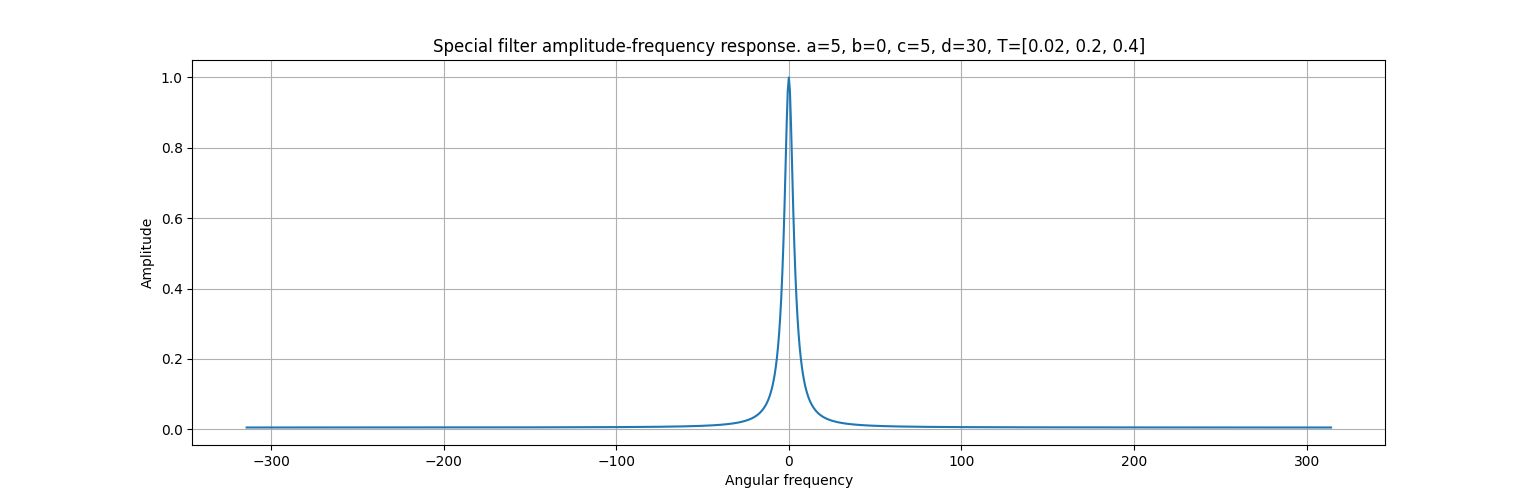
\includegraphics[scale=0.4]{2_fl2_afr.png}
        \captionsetup{skip=0pt}
        \caption{График амплитудно-частотной характеристики фильтра (2).}
        \label{fig:filinafr22}
    \end{figure}
    \begin{figure}[H]
        \centering
        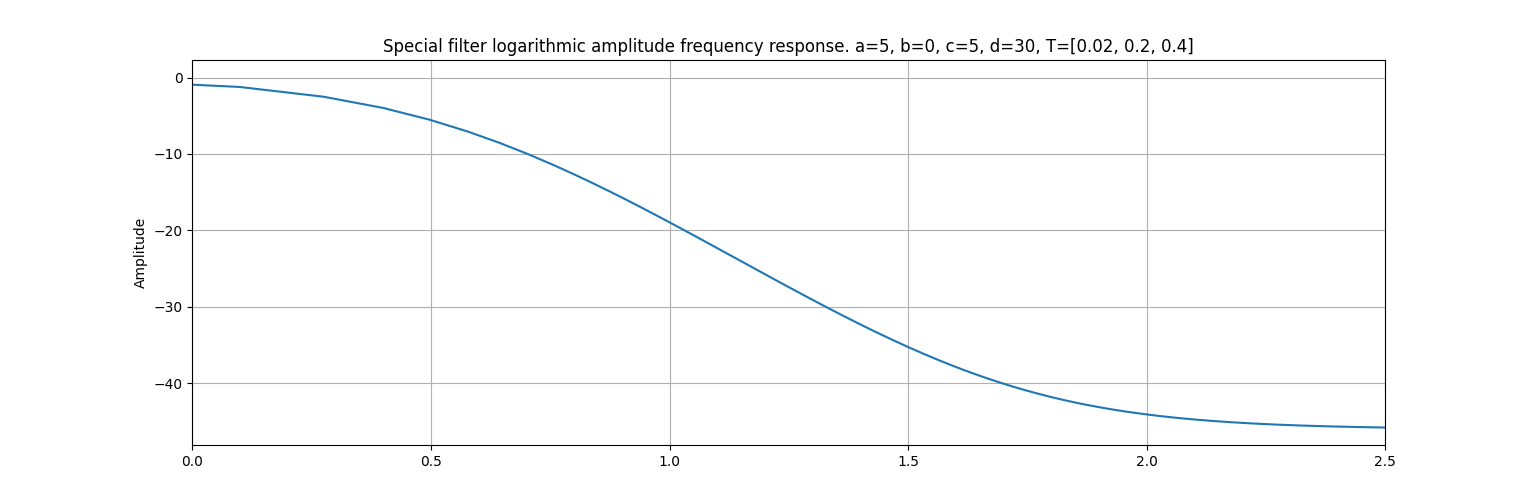
\includegraphics[scale=0.4]{2_fl2_lafr.png}
        \captionsetup{skip=0pt}
        \caption{График логарифмической амплитудно-частотной характеристики фильтра (2).}
        \label{fig:filinlafr22}
    \end{figure}
    \begin{figure}[H]
        \centering
        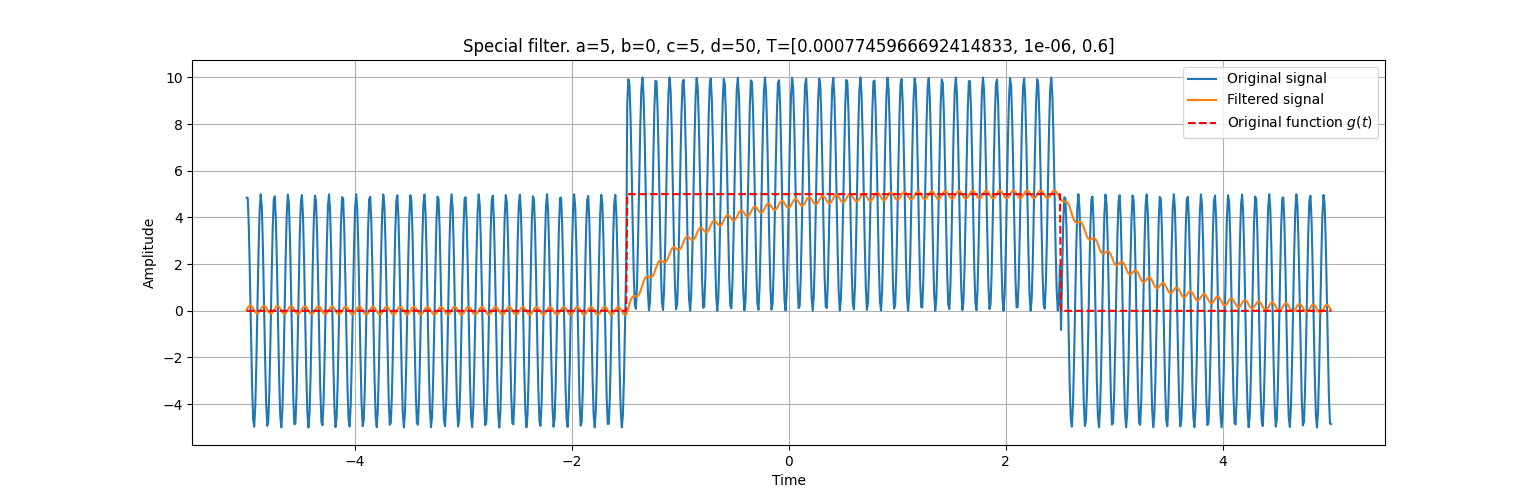
\includegraphics[scale=0.4]{3_fl2.png}
        \captionsetup{skip=0pt}
        \caption{График исходного и фильтрованного сигналов (3).}
        \label{fig:filin23}
    \end{figure}
    \begin{figure}[H]
        \centering
        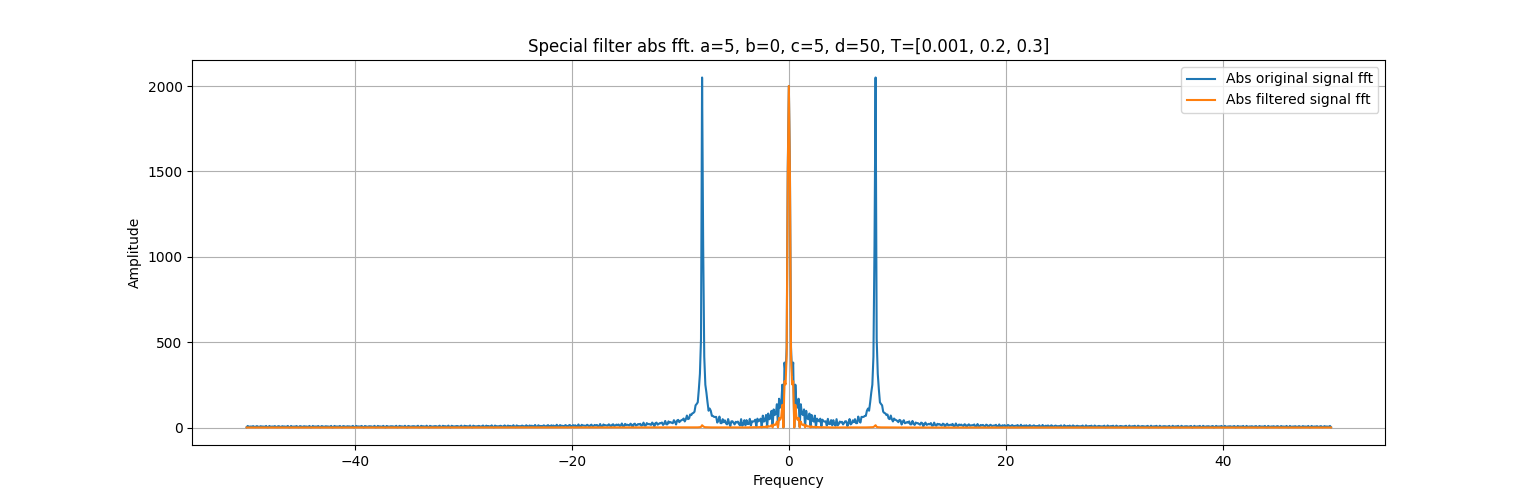
\includegraphics[scale=0.4]{3_fl2_abs.png}
        \captionsetup{skip=0pt}
        \caption{График модулей Фурье-образа исходного и фильтрованного сигналов (3).}
        \label{fig:filinabs23}
    \end{figure}
    \begin{figure}[H]
        \centering
        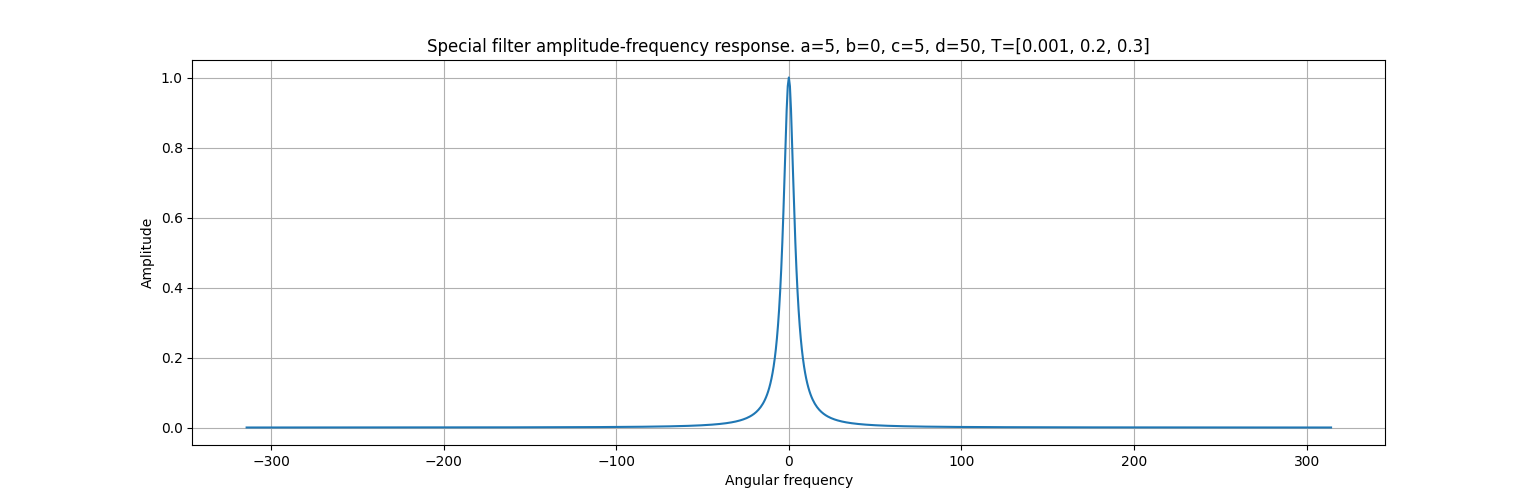
\includegraphics[scale=0.4]{3_fl2_afr.png}
        \captionsetup{skip=0pt}
        \caption{График амплитудно-частотной характеристики фильтра (3).}
        \label{fig:filinafr23}
    \end{figure}
    \begin{figure}[H]
        \centering
        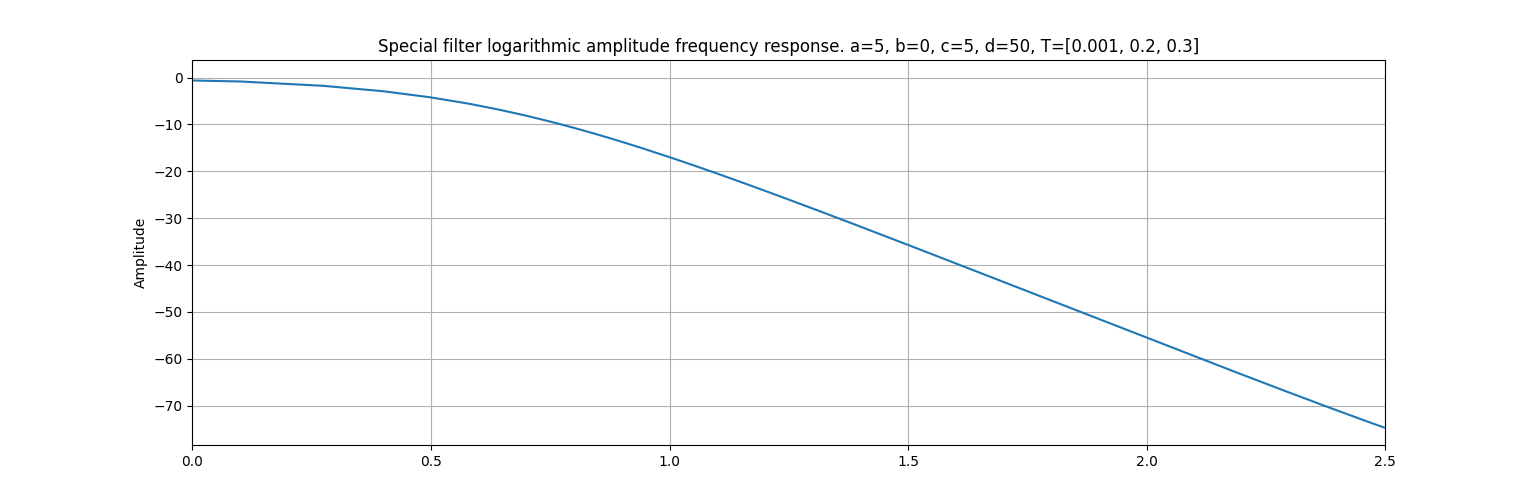
\includegraphics[scale=0.4]{3_fl2_lafr.png}
        \captionsetup{skip=0pt}
        \caption{График логарифмической амплитудно-частотной характеристики фильтра (3).}
        \label{fig:filinlafr23}
    \end{figure}
    \begin{figure}[H]
        \centering
        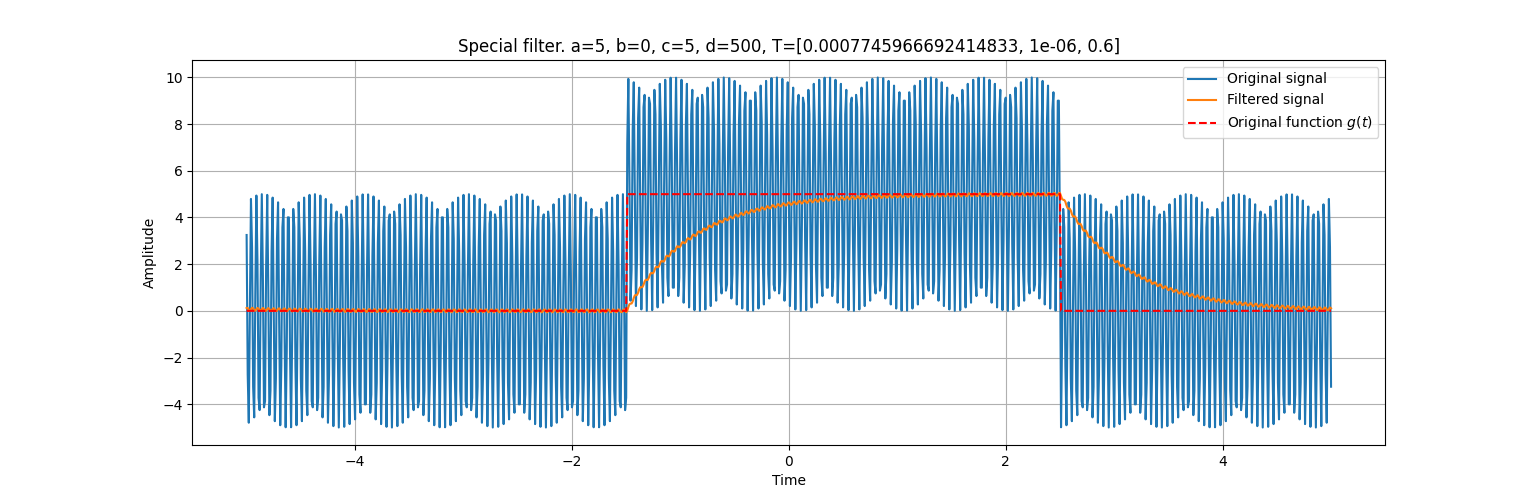
\includegraphics[scale=0.4]{4_fl2.png}
        \captionsetup{skip=0pt}
        \caption{График исходного и фильтрованного сигналов (4).}
        \label{fig:filin24}
    \end{figure}
    \begin{figure}[H]
        \centering
        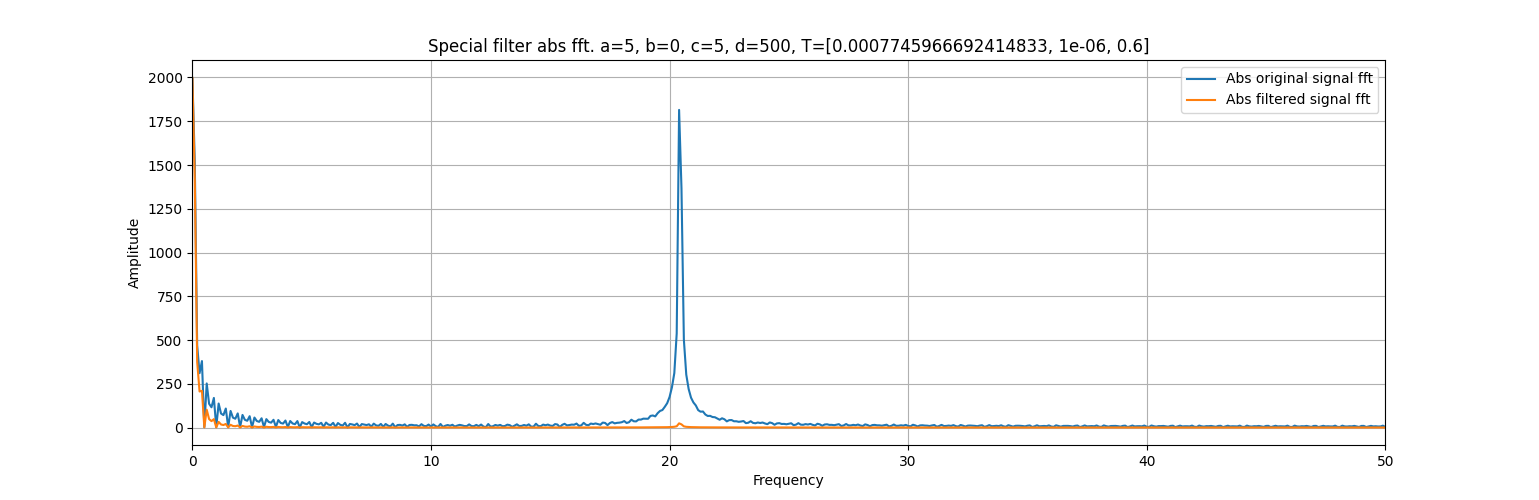
\includegraphics[scale=0.4]{4_fl2_abs.png}
        \captionsetup{skip=0pt}
        \caption{График модулей Фурье-образа исходного и фильтрованного сигналов (4).}
        \label{fig:filinabs24}
    \end{figure}
    \begin{figure}[H]
        \centering
        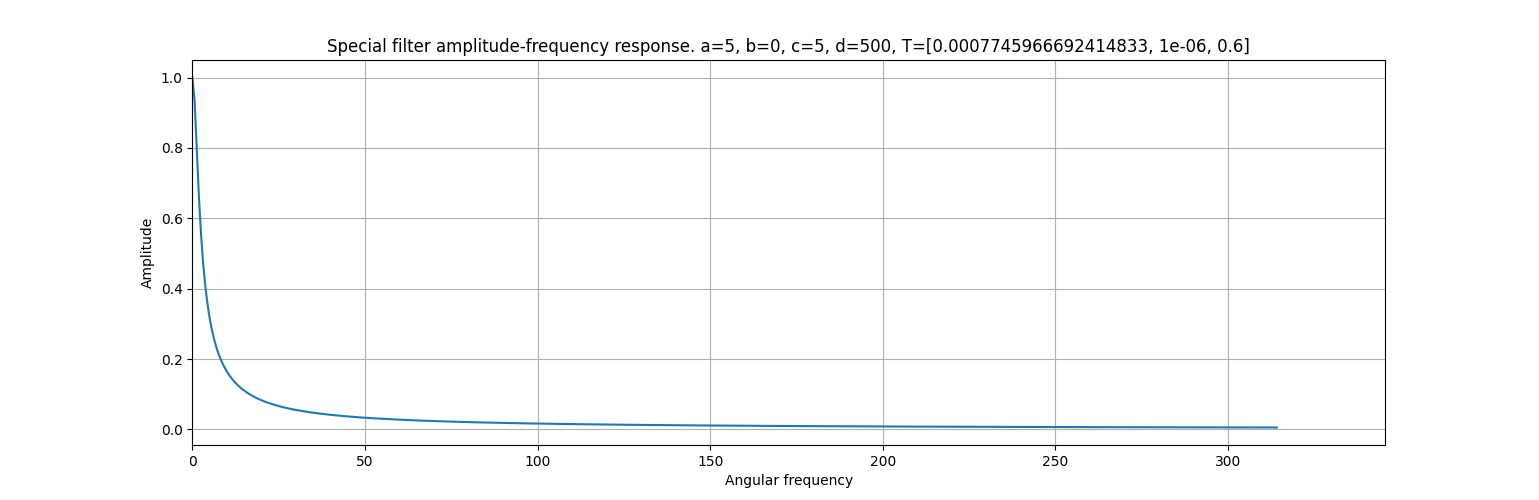
\includegraphics[scale=0.4]{4_fl2_afr.png}
        \captionsetup{skip=0pt}
        \caption{График амплитудно-частотной характеристики фильтра (4).}
        \label{fig:filinafr24}
    \end{figure}
    \begin{figure}[H]
        \centering
        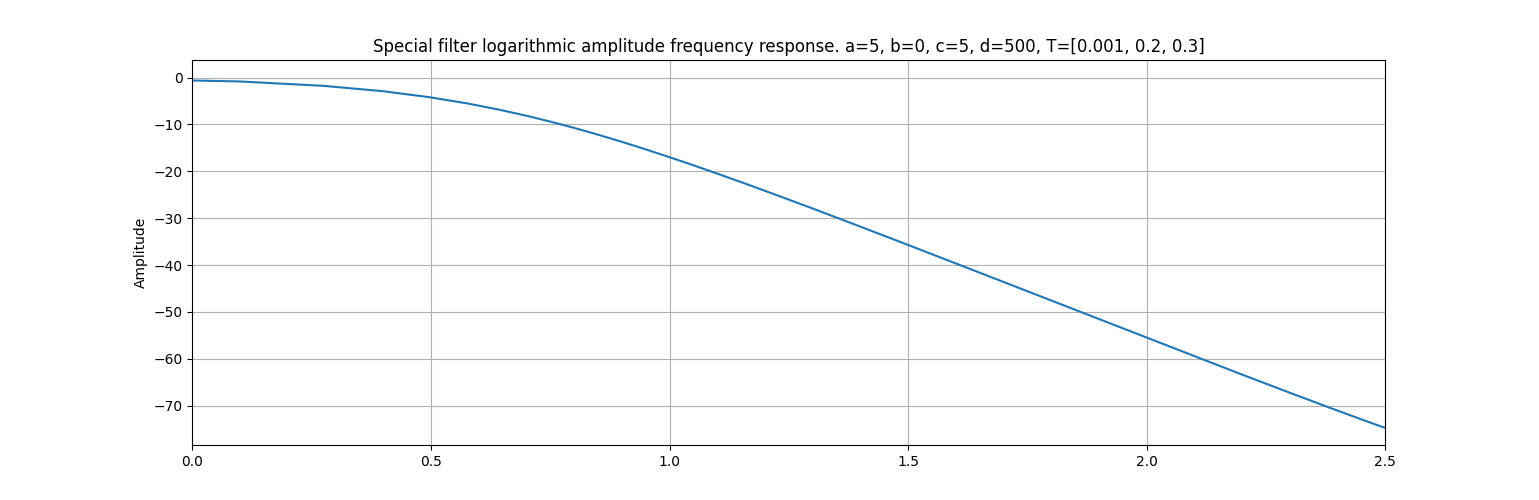
\includegraphics[scale=0.4]{4_fl2_lafr.png}
        \captionsetup{skip=0pt}
        \caption{График логарифмической амплитудно-частотной характеристики фильтра (4).}
        \label{fig:filinlafr24}
    \end{figure}
    \begin{figure}[H]
        \centering
        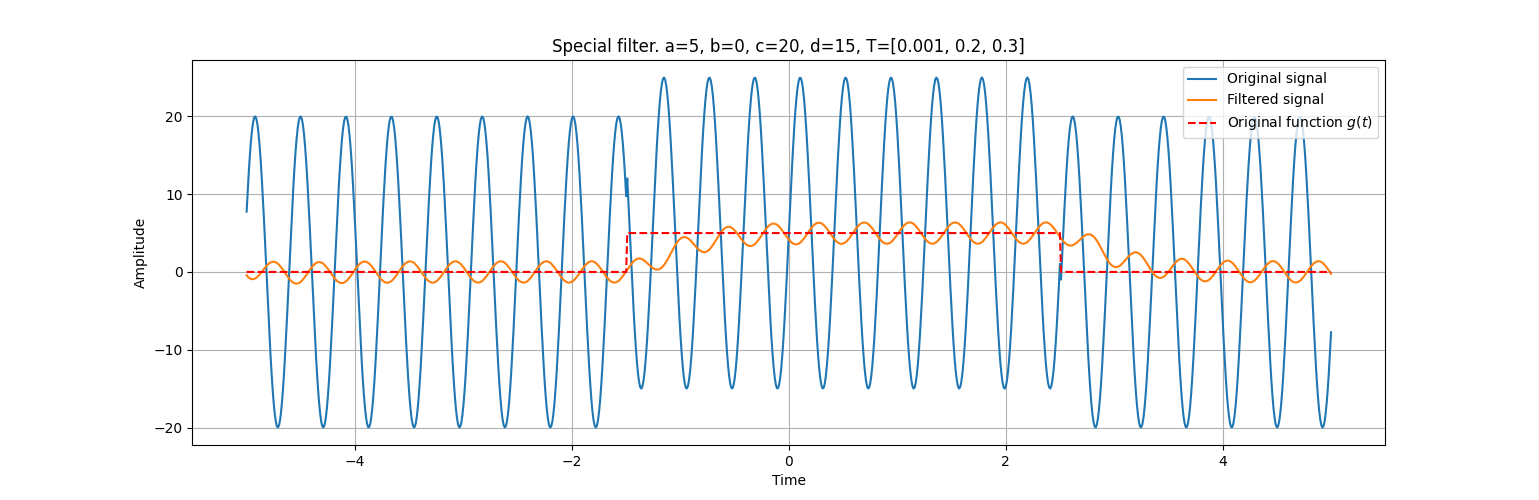
\includegraphics[scale=0.4]{5_fl2.png}
        \captionsetup{skip=0pt}
        \caption{График исходного и фильтрованного сигналов (5).}
        \label{fig:filin25}
    \end{figure}
    \begin{figure}[H]
        \centering
        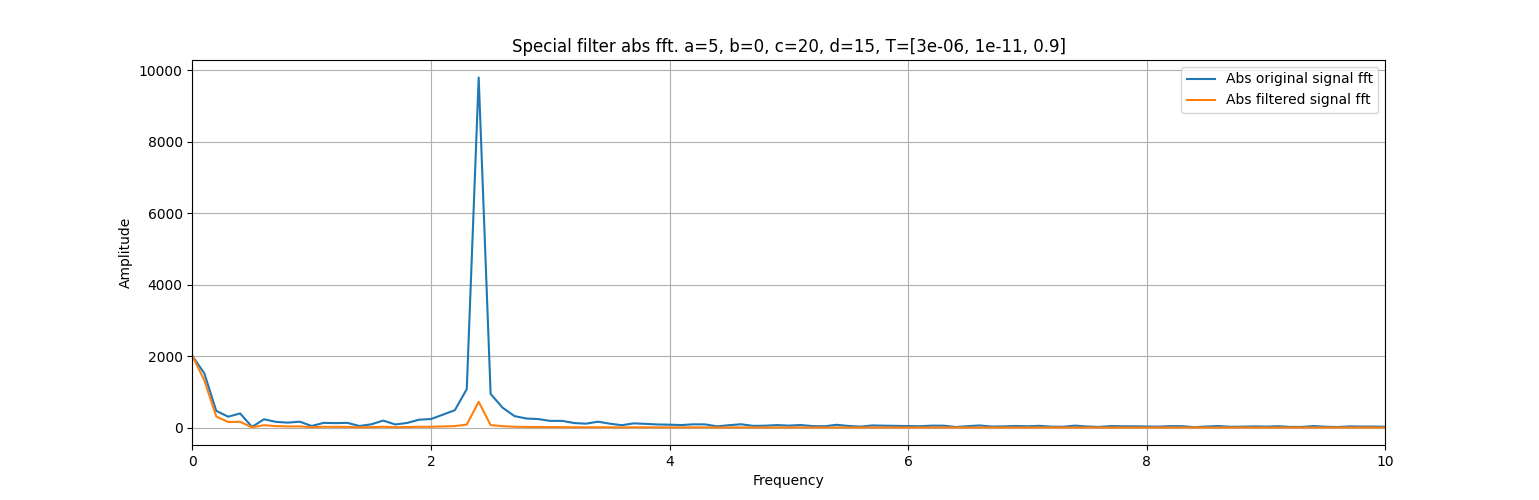
\includegraphics[scale=0.4]{5_fl2_abs.png}
        \captionsetup{skip=0pt}
        \caption{График модулей Фурье-образа исходного и фильтрованного сигналов (5).}
        \label{fig:filinabs25}
    \end{figure}
    \begin{figure}[H]
        \centering
        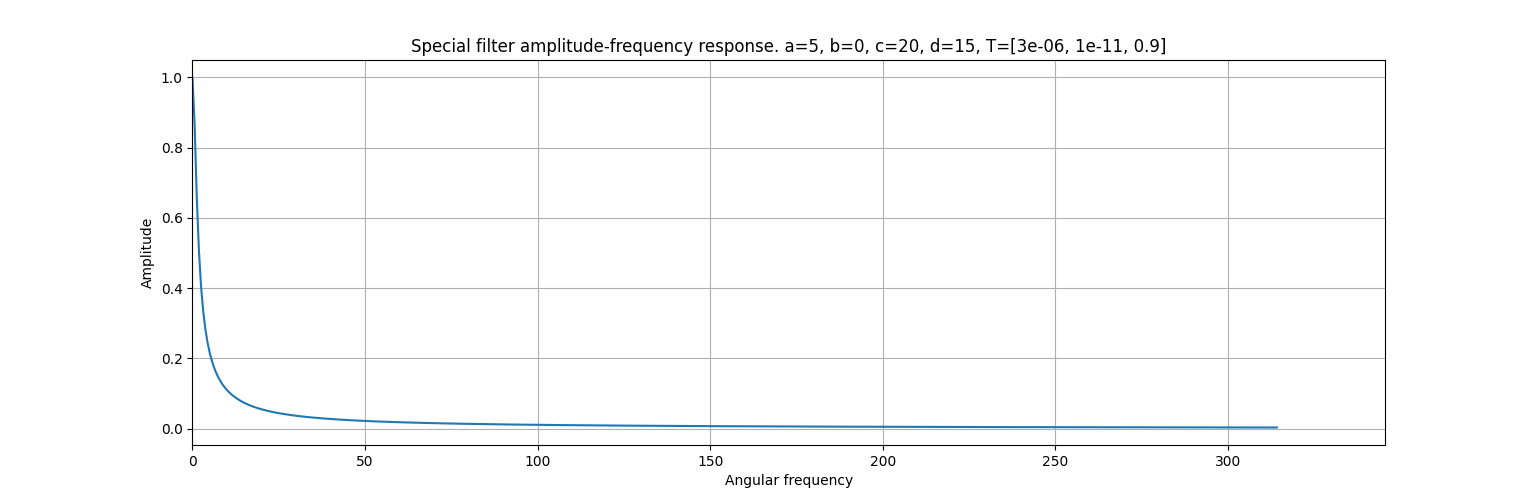
\includegraphics[scale=0.4]{5_fl2_afr.png}
        \captionsetup{skip=0pt}
        \caption{График амплитудно-частотной характеристики фильтра (5).}
        \label{fig:filinafr25}
    \end{figure}
    \begin{figure}[H]
        \centering
        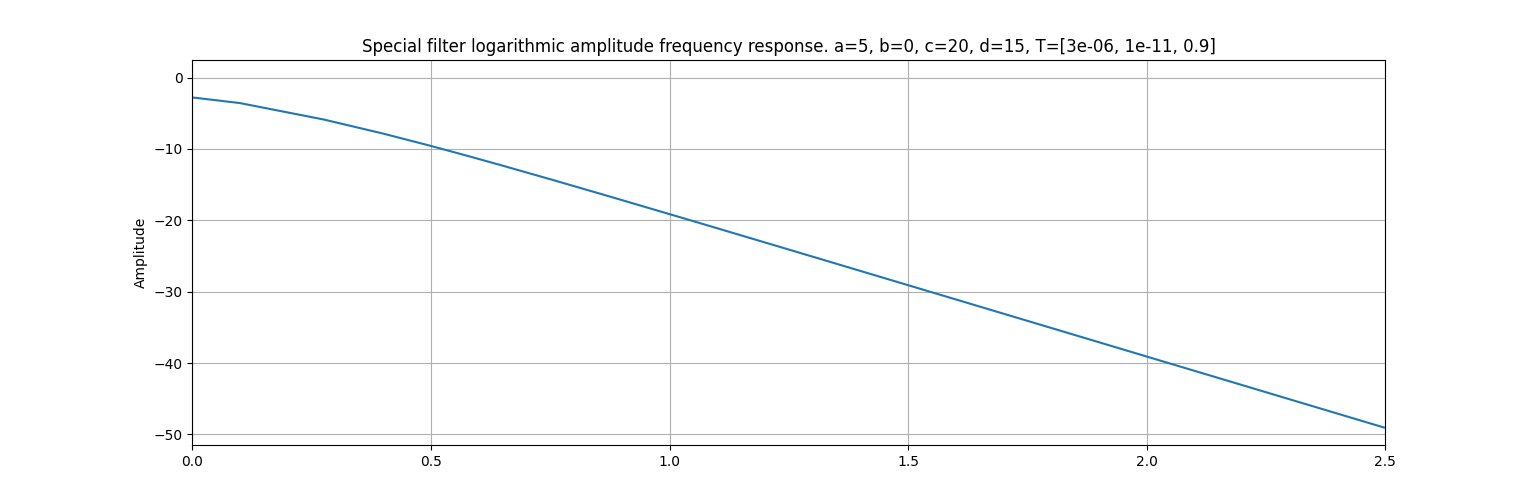
\includegraphics[scale=0.4]{5_fl2_lafr.png}
        \captionsetup{skip=0pt}
        \caption{График логарифмической амплитудно-частотной характеристики фильтра (5).}
        \label{fig:filinlafr25}
    \end{figure}
    \begin{figure}[H]
        \centering
        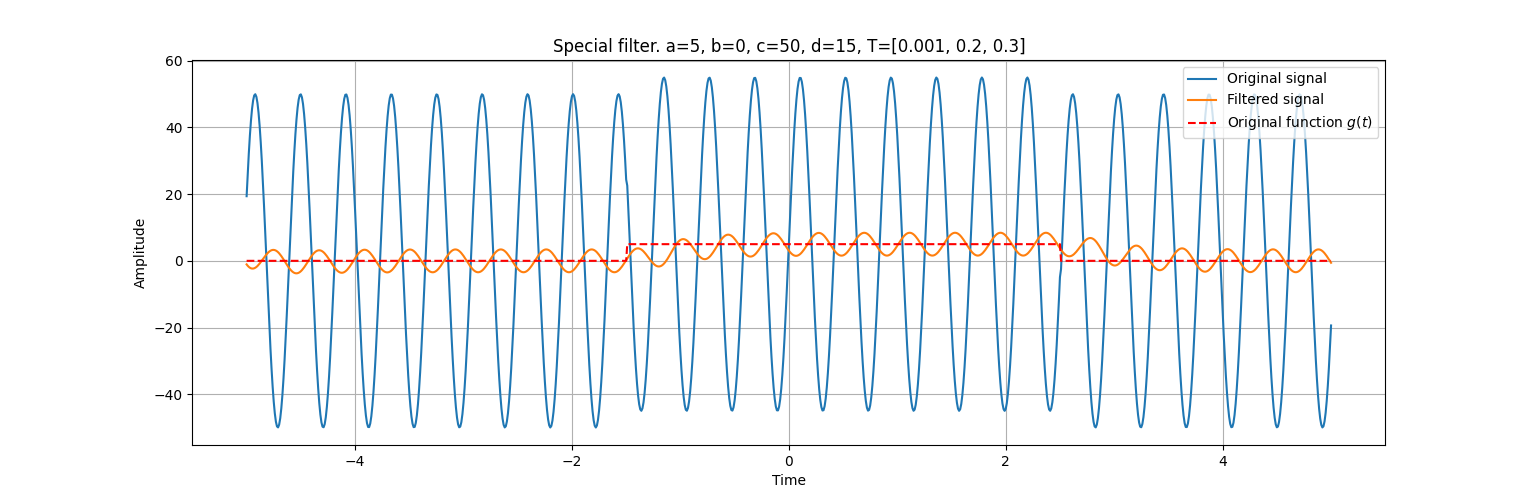
\includegraphics[scale=0.4]{6_fl2.png}
        \captionsetup{skip=0pt}
        \caption{График исходного и фильтрованного сигналов (6).}
        \label{fig:filin26}
    \end{figure}
    \begin{figure}[H]
        \centering
        \includegraphics[scale=0.4]{6_fl2_abs.png}
        \captionsetup{skip=0pt}
        \caption{График модулей Фурье-образа исходного и фильтрованного сигналов (6).}
        \label{fig:filinabs26}
    \end{figure}
    \begin{figure}[H]
        \centering
        \includegraphics[scale=0.4]{6_fl2_afr.png}
        \captionsetup{skip=0pt}
        \caption{График амплитудно-частотной характеристики фильтра (6).}
        \label{fig:filinafr26}
    \end{figure}
    \begin{figure}[H]
        \centering
        \includegraphics[scale=0.4]{6_fl2_lafr.png}
        \captionsetup{skip=0pt}
        \caption{График логарифмической амплитудно-частотной характеристики фильтра (6).}
        \label{fig:filinlafr26}
    \end{figure}
\end{document}